\documentclass[a4paper,11pt]{article}

% ─── Encoding & Language ────────────────────────────────────────────────────
\usepackage[utf8]{inputenc}
\usepackage[T1]{fontenc}
\usepackage[english]{babel}

% ─── Layout ─────────────────────────────────────────────────────────────────
\usepackage[margin=2.5cm]{geometry}
\usepackage{parskip}
\usepackage{enumitem}
% ─── Math ────────────────────────────────────────────────────────────────────
\usepackage{amsmath, amssymb, amsthm}

% ─── Algorithms ──────────────────────────────────────────────────────────────
\usepackage{algorithm}
\usepackage{algpseudocode}
\algrenewcommand\algorithmicindent{1.5em}
\newcommand{\AlgComment}[1]{\hfill\textcolor{gray!70!black}{\textit{// #1}}}

% ─── Graphics & Diagrams ─────────────────────────────────────────────────────
\usepackage{tikz}
\usetikzlibrary{trees, positioning, arrows.meta, shapes.geometric, calc, decorations.pathreplacing}

% ─── Tables ──────────────────────────────────────────────────────────────────
\usepackage{booktabs}
\usepackage{array}
\usepackage{multirow}
\usepackage[table]{xcolor} 
% ─── Colors ──────────────────────────────────────────────────────────────────
\usepackage{xcolor}
\definecolor{keyblue}{RGB}{30, 80, 160}
\definecolor{lightblue}{RGB}{220, 235, 255}
\definecolor{keygreen}{RGB}{20, 130, 60}
\definecolor{lightgreen}{RGB}{220, 245, 225}
\definecolor{keyred}{RGB}{180, 30, 30}
\definecolor{lightyellow}{RGB}{255, 252, 220}
\definecolor{codegray}{rgb}{0.5,0.5,0.5}

% ─── Boxes & Frames ──────────────────────────────────────────────────────────
\usepackage{mdframed}
\usepackage{tcolorbox}
\tcbuselibrary{theorems, skins, breakable}

% ─── Hyperlinks ──────────────────────────────────────────────────────────────
\usepackage{hyperref}
\hypersetup{colorlinks=true, linkcolor=keyblue, urlcolor=keyblue}

% ─── Custom theorem environments ─────────────────────────────────────────────
\newtcbtheorem[number within=section]{definition}{Definition}{
  colback=lightblue, colframe=keyblue,
  fonttitle=\bfseries, breakable
}{def}

\newtcbtheorem[number within=section]{theorem}{Theorem}{
  colback=lightgreen, colframe=keygreen,
  fonttitle=\bfseries, breakable
}{thm}

\newtcbtheorem[number within=section]{remark}{Key point}{
  colback=lightyellow, colframe=orange!70!black,
  fonttitle=\bfseries, breakable
}{rem}

\newtcbtheorem[number within=section]{complexity}{Complexity}{
  colback=gray!10, colframe=gray!60,
  fonttitle=\bfseries, breakable
}{cpl}

\DeclareMathOperator{\depth}{depth}

% ─── Metadata ────────────────────────────────────────────────────────────────
\title{\textbf{Algorithm}\\[0.5em]
       \large Lecture resume BA4 -- EPFL\\
       lecture of Ola Svensson}
\author{Liam Vuilleumier}
\date{2026}

% ─────────────────────────────────────────────────────────────────────────────
\begin{document}
\maketitle
\tableofcontents
\newpage

% ─────────────────────────────────────────────────────────────────────────────
\section{Lecture 1 : Introduction to Algorithm}
\subsection{What is an algorithm?}

An \textbf{algorithm} is a well-defined computational procedure that takes one or more
values as \textbf{input} and produces one or more values as
\textbf{output}: it is a sequence of steps transforming input into output.

We distinguish an algorithm from a \textbf{data structure}, which is a method for
storing and organizing information to facilitate its access and modification.

% ─────────────────────────────────────────────────────────────────────────────
\subsection{Introductory example: arithmetic sum}

\textbf{Problem:} calculate $\displaystyle S = \sum_{i=1}^{n} i$.

\begin{center}
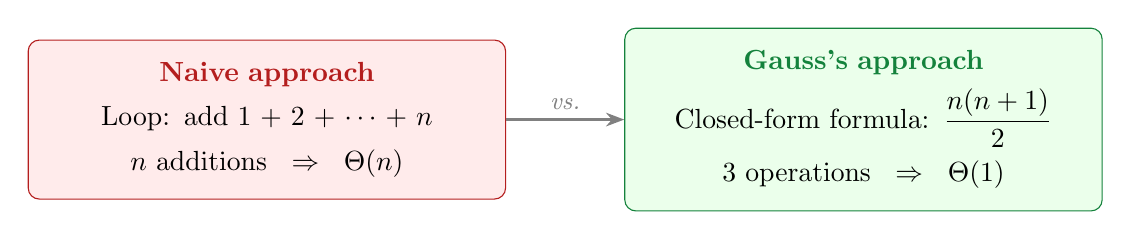
\begin{tikzpicture}[>=Stealth]
  % Naive box
  \node[draw=keyred, fill=red!8, rounded corners, text width=5.5cm, align=center,
        inner sep=8pt] (naive) {
    \textbf{\textcolor{keyred}{Naive approach}}\\[4pt]
    Loop: add $1 + 2 + \cdots + n$\\[4pt]
    $n$ additions \;\;$\Rightarrow$\;\; $\Theta(n)$
  };
  % Smart box
  \node[draw=keygreen, fill=green!8, rounded corners, text width=5.5cm, align=center,
        inner sep=8pt, right=1.5cm of naive] (smart) {
    \textbf{\textcolor{keygreen}{Gauss's approach}}\\[4pt]
    Closed-form formula: $\dfrac{n(n+1)}{2}$\\[4pt]
    3 operations \;\;$\Rightarrow$\;\; $\Theta(1)$
  };
  \draw[->, thick, gray] (naive) -- node[above, font=\small\itshape]{vs.} (smart);
\end{tikzpicture}
\end{center}

% ─────────────────────────────────────────────────────────────────────────────
\subsection{Why does efficiency matter?}

A \emph{slow} computer running a good algorithm will always eventually beat a
\emph{fast} computer running a bad algorithm, as soon as the input size $n$
becomes large enough.

\begin{center}
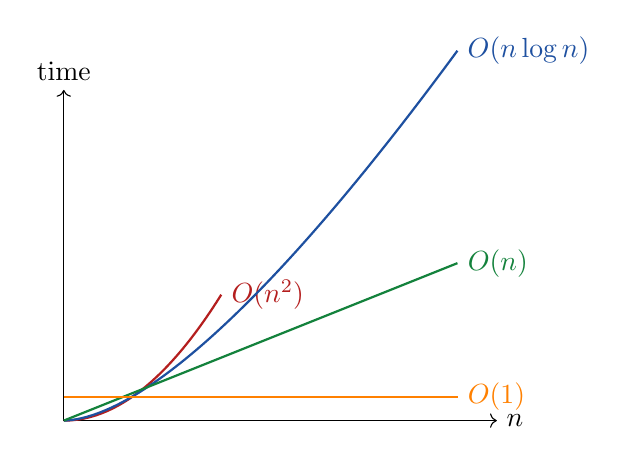
\begin{tikzpicture}
  \begin{scope}
    \draw[->] (0,0) -- (5.5,0) node[right] {$n$};
    \draw[->] (0,0) -- (0,4.2) node[above] {time};
    % O(n^2)
    \draw[keyred, thick, domain=0:2.0, samples=60]
          plot (\x, {0.4*\x*\x}) node[right] {$O(n^2)$};
    % O(n log n)
    \draw[keyblue, thick, domain=0:5, samples=100]
          plot (\x, {0.35*\x*(ln(\x+1)/ln(2)+0.1)}) node[right] {$O(n\log n)$};
    % O(n)
    \draw[keygreen, thick, domain=0:5, samples=60]
          plot (\x, {0.4*\x}) node[right] {$O(n)$};
    % O(1)
    \draw[orange, thick] (0,0.3) -- (5,0.3) node[right] {$O(1)$};
  \end{scope}
\end{tikzpicture}
\end{center}

\begin{tcolorbox}[colback=lightyellow, colframe=orange!70!black, fonttitle=\bfseries,
                  title={Conclusion}]
The \textbf{asymptotic performance} (behavior as $n \to \infty$) is more
decisive than the multiplicative constants related to the hardware.
\end{tcolorbox}

\section{Lecture 2 : sort and analyse complexity}
\subsection{Le problème du tri}

\textbf{Entrée :} une séquence de $n$ nombres $\langle a_1, a_2, \dots, a_n \rangle$.\\
\textbf{Sortie :} une permutation $\langle a'_1, a'_2, \dots, a'_n \rangle$ telle que
$a'_1 \le a'_2 \le \dots \le a'_n$.

% ─────────────────────────────────────────────────────────────────────────────
\subsection{Tri par insertion (\textit{Insertion Sort})}

L'idée est celle du tri d'une main de cartes : on parcourt les éléments un par un et on
insère chaque nouvel élément à sa place correcte parmi ceux déjà triés.

\begin{center}
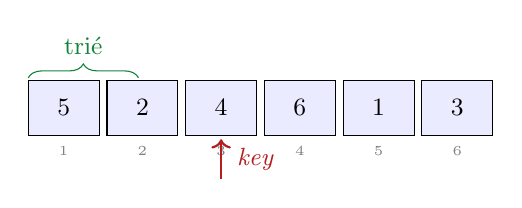
\begin{tikzpicture}[font=\small]
  % Array cells
  \foreach \val/\idx in {5/1,2/2,4/3,6/4,1/5,3/6}{
    \node[draw, minimum width=0.9cm, minimum height=0.7cm,
          fill=blue!8] at (\idx*1.0-0.5, 0) {\val};
    \node[font=\tiny, gray] at (\idx*1.0-0.5, -0.55) {\idx};
  }
  % Arrow showing "key"
  \draw[->, keyred, thick] (2.5, -0.9) -- (2.5, -0.4)
        node[midway, right=2pt, keyred] {\textit{key}};
  % Already sorted bracket
  \draw[decorate, decoration={brace,amplitude=5pt}, keygreen]
        (0.05, 0.38) -- (1.45, 0.38)
        node[midway, above=5pt, keygreen] {trié};
\end{tikzpicture}
\end{center}

\begin{algorithm}[H]
\caption{Insertion-Sort($A$)}
\begin{algorithmic}[1]
\For{$j = 2$ \textbf{to} $A.length$}
    \State $key \leftarrow A[j]$  \AlgComment{élément à insérer}
    \State $i \leftarrow j - 1$
    \While{$i > 0$ \textbf{and} $A[i] > key$}
        \State $A[i+1] \leftarrow A[i]$  \AlgComment{décaler vers la droite}
        \State $i \leftarrow i - 1$
    \EndWhile
    \State $A[i+1] \leftarrow key$  \AlgComment{insérer à la bonne place}
\EndFor
\end{algorithmic}
\end{algorithm}

% ─────────────────────────────────────────────────────────────────────────────
\subsection{Preuve de correction : invariant de boucle}

Pour prouver qu'un algorithme itératif est correct, on utilise un \textbf{invariant de
boucle}, une propriété vérifiée à trois moments clés :

\begin{enumerate}
  \item \textbf{Initialisation} : vraie avant la première itération.
  \item \textbf{Conservation} : si vraie avant une itération, reste vraie avant la suivante.
  \item \textbf{Terminaison} : à la fin de la boucle, l'invariant prouve la correction.
\end{enumerate}

\textbf{Invariant pour le tri par insertion :} au début de chaque itération $j$, le
sous-tableau $A[1 \ldots j-1]$ contient les éléments initialement en $A[1 \ldots j-1]$,
\emph{mais triés}.

% ─────────────────────────────────────────────────────────────────────────────
\subsection{Analyse de complexité (modèle RAM)}

On utilise le modèle \textbf{Random-Access Machine (RAM)} : chaque instruction simple
(arithmétique, accès mémoire, test) prend un temps constant.

\begin{center}
\renewcommand{\arraystretch}{1.3}
\begin{tabular}{lll}
\toprule
\textbf{Cas} & \textbf{Condition} & \textbf{Complexité} \\
\midrule
Meilleur cas & Tableau déjà trié (while ne s'exécute jamais) & $\Theta(n)$ \\
Pire cas     & Tableau trié en ordre inverse & $\Theta(n^2)$ \\
\bottomrule
\end{tabular}
\end{center}

\textbf{Calcul du pire cas :}
\[
  T(n) = \sum_{j=2}^{n} (j-1) = \frac{n(n-1)}{2} = \Theta(n^2)
\]

\begin{tcolorbox}[colback=lightblue, colframe=keyblue, fonttitle=\bfseries,
                  title={Pourquoi se concentrer sur le pire cas ?}]
Il fournit une \textbf{garantie supérieure} sur le temps d'exécution, valable pour toute
entrée possible. C'est la référence standard en analyse d'algorithmes.
\end{tcolorbox}

\section{Lecture 3 : divide to conquer \& Fusion sort}

\subsection{Le paradigme Diviser pour Régner}
Cette approche récursive pour résoudre un problème se décompose en trois étapes :
\begin{enumerate}
    \item \textbf{Diviser} le problème en plusieurs sous-problèmes qui sont des instances plus petites du même problème.
    \item \textbf{Régner} sur les sous-problèmes en les résolvant récursivement. (Cas de base : si le problème est assez petit, on le résout directement).
    \item \textbf{Combiner} les solutions des sous-problèmes pour obtenir la solution du problème original.
\end{enumerate}

\subsection{Tri Fusion (Merge Sort)}
L'algorithme applique ce paradigme au tri :
\begin{itemize}
    \item \textbf{Diviser :} Séparer le tableau de $n$ éléments en deux sous-tableaux de taille $n/2$.
    \item \textbf{Régner :} Trier récursivement les deux sous-tableaux avec \textsc{Merge-Sort}.
    \item \textbf{Combiner :} Fusionner (\textsc{Merge}) les deux sous-tableaux triés pour produire un unique tableau trié.
\end{itemize}

\subsubsection{La procédure Merge (Fusion)}
L'étape clé est la fusion de deux séquences triées.
\begin{itemize}
    \item On compare les têtes des deux listes et on place le plus petit élément dans le tableau de sortie.
    \item Cette opération prend un temps linéaire $\Theta(n)$ où $n$ est le nombre total d'éléments à fusionner.
\end{itemize}

\subsection{Analyse du Tri Fusion}
Soit $T(n)$ le temps pour trier $n$ éléments.
\begin{equation}
    T(n) = 
    \begin{cases} 
    \Theta(1) & \text{si } n = 1 \\
    2T(n/2) + \Theta(n) & \text{si } n > 1 
    \end{cases}
\end{equation}
\begin{itemize}
    \item $2T(n/2)$ correspond à la résolution des deux sous-problèmes.
    \item $\Theta(n)$ correspond au temps de la division et surtout de la fusion (Combiner).
\end{itemize}

En résolvant cette récurrence (par exemple via l'arbre de récursion ou le \textit{Master Theorem} vu plus tard), on obtient :
\[ T(n) = \Theta(n \log n) \]

\textbf{Conclusion :} Pour de grandes valeurs de $n$, le Tri Fusion ($\Theta(n \log n)$) est nettement plus rapide que le Tri par Insertion ($\Theta(n^2)$).

\section{Lecture 4 : Recurence analysis \& Maximum sub-array}
\input{Lecture/Lecture4}

\section{Lecture 5 : matrice multiplication \& heap}
\subsection{Matrix Multiplication}
Given two $n \times n$ matrices $A$ and $B$, the product $C = A \cdot B$ has $c_{ij} = \sum_{k=1}^n a_{ik}b_{kj}$.

\subsubsection{Naive vs. Strassen's Algorithm}
\begin{itemize}
    \item \textbf{Naive Algorithm:} Three nested loops, resulting in $\Theta(n^3)$.
    \item \textbf{Simple Divide-and-Conquer:} Splitting matrices into 4 sub-matrices of size $n/2$. 
    $T(n) = 8T(n/2) + \Theta(n^2) = \Theta(n^3)$. No improvement.
    \item \textbf{Strassen's Algorithm:} Uses algebraic tricks to compute only \textbf{7 multiplications} instead of 8.
    \[ T(n) = 7T(n/2) + \Theta(n^2) \]
    Using Master Theorem Case 1 ($\log_2 7 \approx 2.81$):
    \[ \boxed{T(n) = \Theta(n^{\log_2 7}) \approx \Theta(n^{2.81})} \]
\end{itemize}

\subsection{Heaps and Heapsort}
Heapsort combines the benefits of Merge Sort ($O(n \log n)$) and Insertion Sort (in-place).

\subsubsection{Binary Heap Structure}
A heap is an almost complete binary tree stored in an array.
\begin{itemize}
    \item \textbf{Root:} $A[1]$
    \item \textbf{Max-Heap Property:} $A[\text{Parent}(i)] \ge A[i]$. The largest element is at the root.
    \item \textbf{Height:} A heap of $n$ elements has height $\Theta(\log n)$.
\end{itemize}

\subsubsection{Key Operations}
\subsubsection{Max-Heapify}
Maintains the heap property. If an element is smaller than its children, it "sinks" down the tree.
\begin{itemize}
    \item \textbf{Complexity:} $O(\log n)$.
\end{itemize}

\subsubsection{Build-Max-Heap}
Converts an unordered array into a Max-Heap by calling \textit{Max-Heapify} on all non-leaf nodes.
\begin{itemize}
    \item \textbf{Complexity:} Although it makes $O(n)$ calls to a $\log n$ function, the tighter analysis shows it is \textbf{linear}.
    \[ \boxed{T(n) = \Theta(n)} \]
\end{itemize}

\begin{algorithmic}[1]
\Function{Build-Max-Heap}{$A$}
    \State $A.heap\_size \gets A.length$
    \For{$i \gets \lfloor A.length/2 \rfloor$ \textbf{downto} $1$}
        \State \Call{Max-Heapify}{$A, i$}
    \EndFor
\EndFunction
\end{algorithmic}

\section{Lecture 6 : Heapsort \& priority files}
% Lecture 6: Heapsort & Priority Queues
% (Reminders on matrix multiplication and the heap structure 
% were covered in Lecture 5.)

\subsection{The Heapsort Algorithm}

Heapsort sorts an array \emph{in-place} in $O(n\log n)$ in the worst case.

\begin{enumerate}
  \item \textbf{Build} a max-heap from the input array: $O(n)$.
  \item \textbf{Repeat $n-1$ times:}
    \begin{enumerate}[label=\alph*.]
      \item Exchange the root (maximum) $A[1]$ with the last element $A[heap\_size]$.
      \item Reduce $heap\_size$ by 1 (the exchanged element is in its final position).
      \item Call \textsc{Max-Heapify}$(A, 1)$ to restore the property: $O(\log n)$.
    \end{enumerate}
\end{enumerate}

\begin{center}
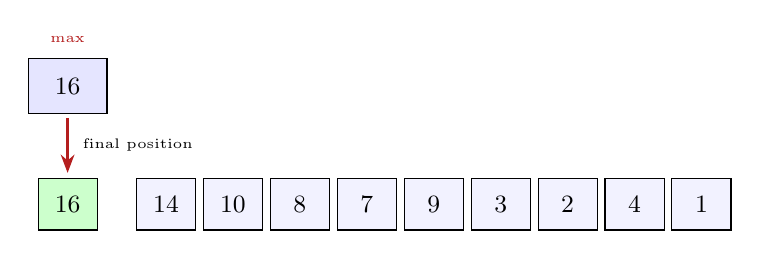
\begin{tikzpicture}[font=\small, >=Stealth]
  % Steps illustration
  \node[draw, fill=blue!10, minimum width=1cm, minimum height=0.7cm] (r) at (0,1.5) {16};
  \node[above=2pt of r, font=\tiny, keyred] {max};
  \foreach \v/\i in {14/1, 10/2, 8/3, 7/4, 9/5, 3/6, 2/7, 4/8, 1/9}{
    \node[draw, fill=blue!5, minimum width=0.75cm, minimum height=0.65cm]
          at (\i*0.85-0.5+0.9, 0) {\v};
  }
  \node[draw, fill=green!20, minimum width=0.75cm, minimum height=0.65cm]
        at (0, 0) {16};
  % Arrow
  \draw[->, thick, keyred] (0, 1.1) -- (0, 0.4);
  \node[right=2pt, font=\tiny] at (0, 0.75) {final position};
\end{tikzpicture}
\end{center}

\begin{complexity}{Heapsort}{heapcplx}
\begin{itemize}[noitemsep]
  \item \textsc{Build-Max-Heap}: $O(n)$.
  \item $n-1$ calls to \textsc{Max-Heapify}: $O(\log n)$ each.
  \item \textbf{Total: $O(n \log n)$ in all cases.}
\end{itemize}
\end{complexity}

% ─────────────────────────────────────────────────────────────────────────────
\subsection{Priority Queues}

A \textbf{(max) priority queue} maintains a dynamic set of elements with keys,
and supports:

\begin{center}
\renewcommand{\arraystretch}{1.3}
\begin{tabular}{lll}
\toprule
\textbf{Operation} & \textbf{Description} & \textbf{Time} \\
\midrule
\textsc{Maximum}$(S)$       & Returns the element with the maximum key & $O(1)$ \\
\textsc{Extract-Max}$(S)$   & Removes and returns the maximum      & $O(\log n)$ \\
\textsc{Increase-Key}$(S,x,k)$ & Increases the key of $x$ to $k$   & $O(\log n)$ \\
\textsc{Insert}$(S,x)$      & Inserts $x$ into $S$                 & $O(\log n)$ \\
\bottomrule
\end{tabular}
\end{center}

\textbf{Implementation}: the binary heap implements all these operations efficiently.

\paragraph{\textsc{Extract-Max}.}
\begin{enumerate}[noitemsep]
  \item Save $A[1]$ (the maximum).
  \item Put $A[heap\_size]$ at the root, reduce $heap\_size$.
  \item Call \textsc{Max-Heapify}$(A,1)$.
\end{enumerate}

\paragraph{\textsc{Increase-Key}$(A, i, k)$.}
After updating $A[i] \leftarrow k$, move up the tree as long as the max-heap 
property is violated (the element "floats" upward).

\begin{tcolorbox}[colback=lightblue, colframe=keyblue, fonttitle=\bfseries,
                  title={Application: Priority Queue}]
Used in graph algorithms (Dijkstra, Prim) to efficiently extract the next 
vertex to be processed.
\end{tcolorbox}

\section{Lecture 7 : elementary data structure }
\subsection{Dynamic Sets}

Data structures are used to implement \textbf{dynamic sets}.
Operations are grouped into two categories:

\begin{itemize}
  \item \textbf{Modification}: Insert, Delete, \dots
  \item \textbf{Query}: Search, Minimum, Maximum, \dots
\end{itemize}

% ─────────────────────────────────────────────────────────────────────────────
\subsection{Stacks -- LIFO}

A stack follows the \textbf{LIFO} (\textit{Last-In, First-Out}) principle: last in,
first out, like a stack of plates.

\begin{center}
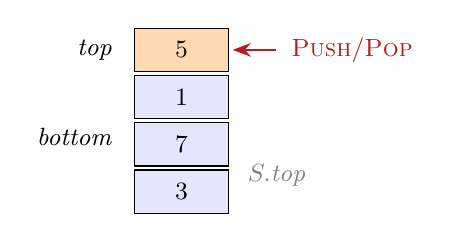
\begin{tikzpicture}[font=\small, >=Stealth]
  \foreach \v/\i in {3/1, 7/2, 1/3}{
    \node[draw, fill=blue!10, minimum width=1.2cm, minimum height=0.55cm]
          at (0, \i*0.6-0.3) {\v};
  }
  \node[draw, fill=orange!30, minimum width=1.2cm, minimum height=0.55cm]
        at (0, 4*0.6-0.3) {5};
  \draw[->, thick, keyred] (1.2, 4*0.6-0.3) -- (0.65, 4*0.6-0.3)
        node[left=0pt]{}; 
  \node[right=2pt, keyred] at (1.2, 4*0.6-0.3) {\textsc{Push}/\textsc{Pop}};
  \node[left=4pt] at (-0.6, 1) {\textit{bottom}};
  \node[left=4pt] at (-0.6, 4*0.6-0.3) {\textit{top}};
  \node[right=2pt, gray] at (0.65, 0.5) {$S.\mathit{top}$};
\end{tikzpicture}
\end{center}

\begin{itemize}
  \item \textsc{Push}$(S, x)$: pushes $x$ onto the top. $O(1)$.
  \item \textsc{Pop}$(S)$: removes and returns the top element. $O(1)$.
  \item \textsc{Stack-Empty}$(S)$: tests if $S.\mathit{top} = 0$. $O(1)$.
\end{itemize}

% ─────────────────────────────────────────────────────────────────────────────
\subsection{Queues -- FIFO}

A queue follows the \textbf{FIFO} (\textit{First-In, First-Out}) principle: first in,
first out, like a waiting line.

\begin{center}
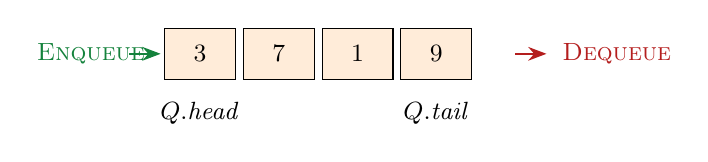
\begin{tikzpicture}[font=\small, >=Stealth]
  \foreach \v/\i in {3/0, 7/1, 1/2, 9/3}{
    \node[draw, fill=orange!15, minimum width=0.9cm, minimum height=0.65cm]
          at (\i*1.0, 0) {\v};
  }
  \draw[->, thick, keygreen] (-0.9, 0) -- (-0.5, 0)
        node[left=2pt, keygreen]{\textsc{Enqueue}};
  \draw[->, thick, keyred] (3.5+0.5, 0) -- (3.5+0.9, 0)
        node[right=2pt, keyred]{\textsc{Dequeue}};
  \node[below=4pt] at (0, -0.35) {\small$Q.\mathit{head}$};
  \node[below=4pt] at (3, -0.35) {\small$Q.\mathit{tail}$};
\end{tikzpicture}
\end{center}

\begin{itemize}
  \item \textsc{Enqueue}$(Q, x)$: adds $x$ to the tail. $O(1)$.
  \item \textsc{Dequeue}$(Q)$: removes and returns the head element. $O(1)$.
\end{itemize}

% ─────────────────────────────────────────────────────────────────────────────
\subsection{Linked Lists}

Linear order is determined by \textbf{pointers} stored in each object
(and not by array indices).

\begin{center}
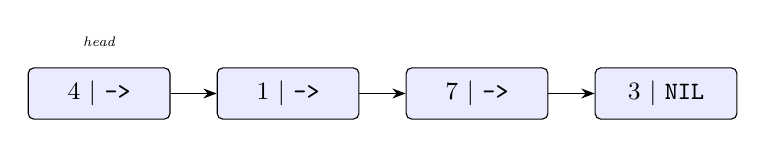
\begin{tikzpicture}[font=\small, >=Stealth,
    node/.style={draw, fill=blue!8, minimum width=1.8cm, minimum height=0.65cm,
                  rounded corners=2pt}]
  \node[node] (a) at (0,0) {4 $|$ \texttt{->}};
  \node[node] (b) at (2.4,0) {1 $|$ \texttt{->}};
  \node[node] (c) at (4.8,0) {7 $|$ \texttt{->}};
  \node[node] (d) at (7.2,0) {3 $|$ \texttt{NIL}};
  \draw[->] (a.east) -- (b.west);
  \draw[->] (b.east) -- (c.west);
  \draw[->] (c.east) -- (d.west);
  \node[above=4pt of a, font=\tiny\itshape] {head};
\end{tikzpicture}
\end{center}

\begin{center}
\renewcommand{\arraystretch}{1.25}
\begin{tabular}{lll}
\toprule
\textbf{Operation} & \textbf{Time} & \textbf{Remark} \\
\midrule
\textsc{List-Search}$(L, k)$  & $O(n)$ & Sequential traversal \\
\textsc{List-Insert}$(L, x)$  & $O(1)$ & Insertion at the head \\
\textsc{List-Delete}$(L, x)$  & $O(1)$ & If pointer already known (doubly linked list) \\
\bottomrule
\end{tabular}
\end{center}

\textbf{Sentinels:} a dummy object \texttt{L.nil} represents both ends
of the list simultaneously, simplifying boundary cases (no \texttt{NULL} testing).

\subsubsection{Example: reversing a list in $\Theta(n)$ time, $\Theta(1)$ space}

\begin{algorithm}[H]
\caption{Reverse-List($L$)}
\begin{algorithmic}[1]
\State $prev \leftarrow \textsc{NIL}$
\State $curr \leftarrow L.head$
\While{$curr \ne \textsc{NIL}$}
    \State $next \leftarrow curr.next$
    \State $curr.next \leftarrow prev$   \AlgComment{reverse the link}
    \State $prev \leftarrow curr$
    \State $curr \leftarrow next$
\EndWhile
\State $L.head \leftarrow prev$
\end{algorithmic}
\end{algorithm}

\begin{center}
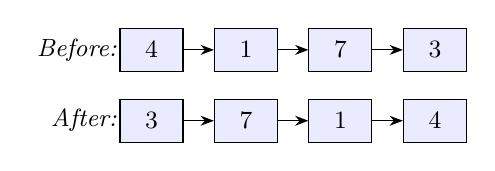
\begin{tikzpicture}[font=\small, >=Stealth,
    node/.style={draw, fill=blue!8, minimum width=0.8cm, minimum height=0.55cm}]
  % Before
  \node[left] at (-0.3, 0.9) {\small\textit{Before:}};
  \foreach \v/\i in {4/0, 1/1, 7/2, 3/3}{
    \node[node] (\i) at (\i*1.2, 0.9) {\v};
  }
  \draw[->] (0.east)--(1.west); \draw[->] (1.east)--(2.west);
  \draw[->] (2.east)--(3.west);
  % After
  \node[left] at (-0.3, 0) {\small\textit{After:}};
  \foreach \v/\i in {3/0, 7/1, 1/2, 4/3}{
    \node[node] (\i r) at (\i*1.2, 0) {\v};
  }
  \draw[->] (0r.east)--(1r.west); \draw[->] (1r.east)--(2r.west);
  \draw[->] (2r.east)--(3r.west);
\end{tikzpicture}
\end{center}

% ─────────────────────────────────────────────────────────────────────────────
\subsection{Conclusion on Elementary Structures}

\begin{tcolorbox}[colback=lightyellow, colframe=orange!70!black, fonttitle=\bfseries,
                  title={Strengths and Limitations}]
Stacks, queues, and linked lists excel at $O(1)$ insertions/deletions,
but are \textbf{poor for searching} ($O(n)$). For fast searching,
more sophisticated structures are needed (trees, hash tables).
\end{tcolorbox}

\section{Lecture 8 : binary tree of research \& dynamic programming}
% ══════════════════════════════════════════════
\subsection{Motivation : le jeu du devin}

Ola pense à un entier entre 1 et 15. À chaque devinette, il répond
\emph{correct}, \emph{plus petit} ou \emph{plus grand}.

\textbf{Stratégie optimale :} toujours deviner le milieu de l'intervalle restant.
Cela garantit de trouver n'importe quel nombre en au plus $\lceil\log_2 15\rceil = 4$
questions. Cette stratégie s'encode naturellement sous la forme d'un arbre :

\begin{center}
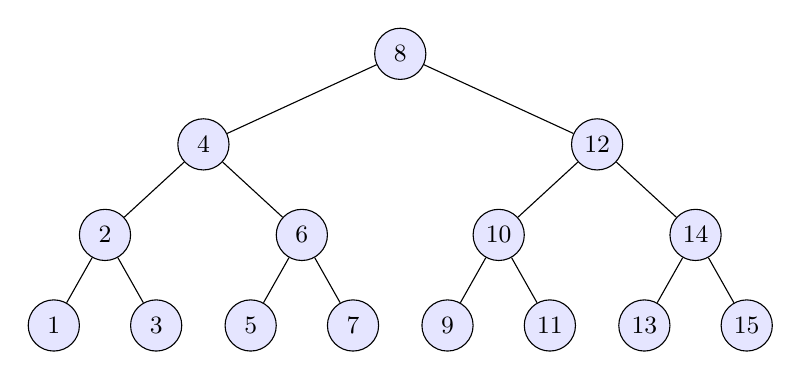
\begin{tikzpicture}[
  level distance=1.15cm,
  level 1/.style={sibling distance=5cm},
  level 2/.style={sibling distance=2.5cm},
  level 3/.style={sibling distance=1.3cm},
  every node/.style={circle, draw, fill=blue!10,
                     inner sep=1pt, minimum size=0.65cm, font=\small}
]
\node {8}
  child { node {4}
    child { node {2}
      child { node {1} }
      child { node {3} }
    }
    child { node {6}
      child { node {5} }
      child { node {7} }
    }
  }
  child { node {12}
    child { node {10}
      child { node {9} }
      child { node {11} }
    }
    child { node {14}
      child { node {13} }
      child { node {15} }
    }
  };
\end{tikzpicture}
\end{center}

% ══════════════════════════════════════════════
\subsection{Définition et propriété fondamentale}

\begin{definition}{Arbre binaire de recherche (ABR)}{bst}
Un \textbf{ABR} est un arbre binaire $T$ où chaque nœud $x$ vérifie :
\begin{itemize}[noitemsep]
  \item Si $y$ est dans le \emph{sous-arbre gauche} de $x$ :
        $y.\mathit{key} < x.\mathit{key}$.
  \item Si $y$ est dans le \emph{sous-arbre droit} de $x$ :
        $y.\mathit{key} \ge x.\mathit{key}$.
\end{itemize}
La \textbf{hauteur} $h$ est le nombre d'arêtes du plus long chemin racine–feuille.
\end{definition}

\begin{center}
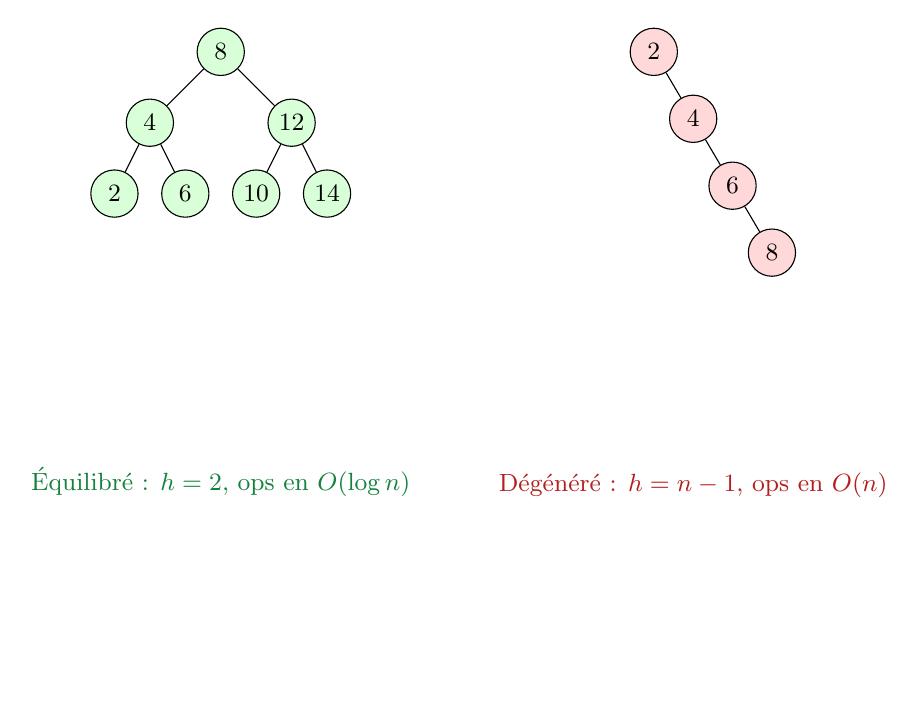
\begin{tikzpicture}[font=\small]
  % Balanced BST
  \begin{scope}[
    level distance=0.9cm,
    level 1/.style={sibling distance=1.8cm},
    level 2/.style={sibling distance=0.9cm},
    every node/.style={circle, draw, fill=green!15,
                       inner sep=1pt, minimum size=0.6cm}]
    \node at (0,0) {8}
      child { node {4}
        child { node {2} }
        child { node {6} }
      }
      child { node {12}
        child { node {10} }
        child { node {14} }
      };
    \node[draw=none, fill=none, below=0.1cm, keygreen] at (0,-2.9)
          {Équilibré : $h = 2$, ops en $O(\log n)$};
  \end{scope}
  % Degenerate BST
  \begin{scope}[xshift=5.5cm,
    level distance=0.85cm,
    level 1/.style={sibling distance=1cm},
    every node/.style={circle, draw, fill=red!15,
                       inner sep=1pt, minimum size=0.6cm}]
    \node at (0,0) {2}
      child[missing]{}
      child { node {4}
        child[missing]{}
        child { node {6}
          child[missing]{}
          child { node {8} }
        }
      };
    \node[draw=none, fill=none, below=0.1cm, keyred] at (0.5,-2.9)
          {Dégénéré : $h = n-1$, ops en $O(n)$};
  \end{scope}
\end{tikzpicture}
\end{center}

\begin{complexity}{Toutes les opérations sur un ABR}{bstcplx}
Recherche, insertion, suppression, min, max, successeur, prédécesseur :
toutes en $O(h)$. Pour un arbre équilibré : $h = O(\log n)$.
\end{complexity}

% ══════════════════════════════════════════════
\subsection{Requêtes sur un ABR}

\subsubsection{Recherche}

\begin{algorithm}[H]
\caption{BST-Search($T$, $k$)}
\begin{algorithmic}[1]
\State $x \leftarrow T.\mathit{root}$
\While{$x \ne \textsc{NIL}$ \textbf{and} $k \ne x.\mathit{key}$}
  \If{$k < x.\mathit{key}$}  \State $x \leftarrow x.\mathit{left}$
  \Else                       \State $x \leftarrow x.\mathit{right}$
  \EndIf
\EndWhile
\State \Return $x$
\end{algorithmic}
\end{algorithm}

\subsubsection{Minimum, Maximum, Successeur}

\begin{theorem}{Localisation de min/max}{minmax}
\begin{itemize}[noitemsep]
  \item Le \textbf{minimum} est le nœud le plus à \emph{gauche}.
  \item Le \textbf{maximum} est le nœud le plus à \emph{droite}.
\end{itemize}
\end{theorem}

Le \textbf{successeur} de $x$ (plus petite clé $> x.\mathit{key}$) se trouve :
\begin{enumerate}[noitemsep]
  \item Si $x$ a un sous-arbre droit : c'est le \emph{minimum} du sous-arbre droit.
  \item Sinon : remonter jusqu'au premier ancêtre $y$ tel que $x$ est dans le sous-arbre
        \emph{gauche} de $y$.
\end{enumerate}

% ══════════════════════════════════════════════
\subsection{Parcours d'un ABR}

\begin{center}
\renewcommand{\arraystretch}{1.3}
\begin{tabular}{llll}
\toprule
\textbf{Parcours} & \textbf{Ordre} & \textbf{Résultat (ex.)} & \textbf{Utilité} \\
\midrule
Infixe (inorder)    & gauche, racine, droite & $1,2,\ldots,n$ (trié !) & Tri \\
Préfixe (preorder)  & racine, gauche, droite & racine en premier & Copie \\
Postfixe (postorder)& gauche, droite, racine & racine en dernier & Suppression \\
\bottomrule
\end{tabular}
\end{center}

\begin{remark}{Parcours infixe et tri}{inorder}
Le parcours infixe d'un ABR produit toujours les clés en \textbf{ordre croissant}
(propriété directe de la définition de l'ABR). Complexité : $\Theta(n)$.
\end{remark}

% ══════════════════════════════════════════════
\subsection{Modifications d'un ABR}

\subsubsection{Insertion}

Chercher $z.\mathit{key}$ jusqu'à atteindre \textsc{NIL}, puis insérer $z$ à cet endroit.
Complexité : $O(h)$.

\subsubsection{Suppression}

Trois cas selon le nombre d'enfants du nœud $z$ à supprimer :

\begin{center}
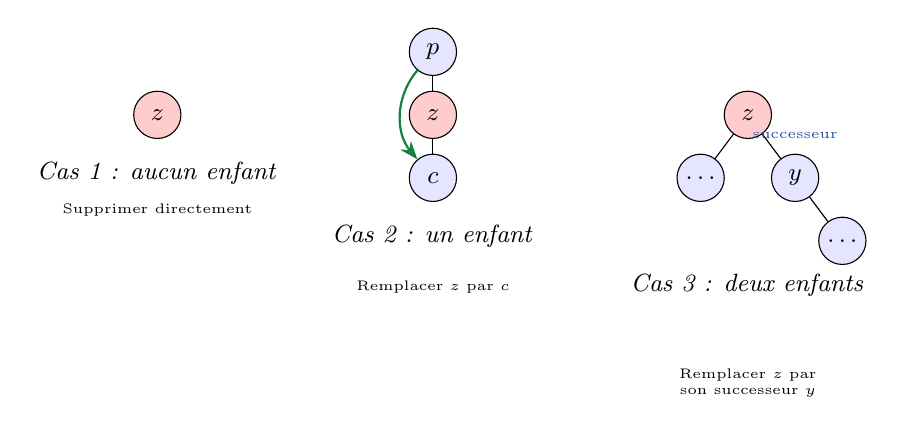
\begin{tikzpicture}[font=\small, >=Stealth,
    node/.style={circle, draw, fill=blue!10,
                 inner sep=1pt, minimum size=0.6cm}]
  % Case 1: no children
  \begin{scope}
    \node[node, fill=red!20] (z1) at (0,0) {$z$};
    \node[draw=none, below=5pt of z1] {\textit{Cas 1 : aucun enfant}};
    \node[draw=none, below=20pt of z1, font=\tiny] {Supprimer directement};
  \end{scope}
  % Case 2: one child
  \begin{scope}[xshift=3.5cm]
    \node[node] (p2) at (0,0.8) {$p$};
    \node[node, fill=red!20] (z2) at (0,0) {$z$};
    \node[node] (c2) at (0,-0.8) {$c$};
    \draw (p2)--(z2)--(c2);
    \draw[->, keygreen, thick] (p2) to[bend right=40] (c2);
    \node[draw=none, below=5pt of c2] {\textit{Cas 2 : un enfant}};
    \node[draw=none, below=25pt of c2, font=\tiny] {Remplacer $z$ par $c$};
  \end{scope}
  % Case 3: two children
  \begin{scope}[xshift=7.5cm,
    level distance=0.8cm,
    level 1/.style={sibling distance=1.2cm}]
    \node[node, fill=red!20] (z3) at (0,0) {$z$}
      child { node[node] {$\ldots$} }
      child { node[node] (succ) {$y$}
        child[missing]{}
        child { node[node] {$\ldots$} }
      };
    \node[above=2pt of succ, font=\tiny, keyblue] {successeur};
    \node[draw=none, below=0.3cm] at (0,-1.6) {\textit{Cas 3 : deux enfants}};
    \node[draw=none, below=1.5cm, font=\tiny, align=center] at (0,-1.6)
          {Remplacer $z$ par\\son successeur $y$};
  \end{scope}
\end{tikzpicture}
\end{center}

% ══════════════════════════════════════════════
\subsection{Bilan des opérations sur un ABR}

\begin{center}
\renewcommand{\arraystretch}{1.35}
\begin{tabular}{lcc}
\toprule
\textbf{Opération} & \textbf{Temps} & \textbf{Idée clé} \\
\midrule
Recherche              & $O(h)$      & Suivre gauche/droite selon la clé \\
Minimum / Maximum      & $O(h)$      & Nœud le plus à gauche/droite \\
Successeur / Préd.     & $O(h)$      & Min du s.a. droit, ou premier ancêtre \\
Insertion              & $O(h)$      & Phase de recherche + insertion feuille \\
Suppression            & $O(h)$      & 3 cas ; utilise \textsc{Transplant} \\
Parcours infixe        & $\Theta(n)$ & Visite chaque nœud une fois \\
\bottomrule
\end{tabular}
\end{center}

\begin{remark}{Équilibrage}{balance}
Dans le pire cas $h = \Theta(n)$ (arbre dégénéré). Les arbres auto-équilibrés
(AVL, rouge-noir) maintiennent $h = O(\log n)$, garantissant $O(\log n)$ par opération.
\end{remark}

% ══════════════════════════════════════════════
\subsection{Comparaison des structures de données}

\begin{center}
\renewcommand{\arraystretch}{1.4}
\begin{tabular}{lcccc}
\toprule
\textbf{Structure}   & \textbf{Capacité} & \textbf{Insertion} & \textbf{Suppression} & \textbf{Recherche} \\
\midrule
Pile / File (tableau)  & fixe    & $O(1)$       & $O(1)$       & $O(n)$ \\
Liste chaînée          & dynamique & $O(1)$     & $O(1)$       & $O(n)$ \\
ABR équilibré          & dynamique & $O(\log n)$ & $O(\log n)$ & $O(\log n)$ \\
\bottomrule
\end{tabular}
\end{center}

% ══════════════════════════════════════════════════════════════════════════════
\section*{Programmation Dynamique}
\addcontentsline{toc}{subsection}{Programmation Dynamique}
% ══════════════════════════════════════════════════════════════════════════════

\subsection{Paradigme et idée centrale}

\begin{definition}{Programmation dynamique (PD)}{dp}
La \textbf{programmation dynamique} est un paradigme algorithmique (pas une
fonctionnalité de langage). Son principe :
\begin{center}
  \textbf{Mémoriser les calculs déjà effectués pour éviter de les refaire.}
\end{center}
Cela permet de transformer des algorithmes exponentiels en algorithmes polynomiaux.
\end{definition}

Un algorithme DP repose sur deux propriétés :
\begin{enumerate}
  \item \textbf{Sous-structure optimale} : la solution optimale d'un problème contient les
        solutions optimales de ses sous-problèmes.
  \item \textbf{Sous-problèmes répétés} : un algorithme récursif naïf recalcule les mêmes
        sous-problèmes un nombre exponentiel de fois.
\end{enumerate}

\textbf{Deux stratégies d'implémentation :}
\begin{itemize}
  \item \textbf{Top-down avec mémoïsation} : récursion + table de résultats.
  \item \textbf{Bottom-up} : remplir la table des petits sous-problèmes vers les grands.
\end{itemize}

% ══════════════════════════════════════════════
\subsection{Premier exemple : nombres de Fibonacci}

\[
  F_0 = 1,\quad F_1 = 1,\quad F_n = F_{n-1} + F_{n-2} \quad (n \ge 2).
\]

\subsubsection{Récursion naïve : arbre de calcul exponentiel}

\begin{center}
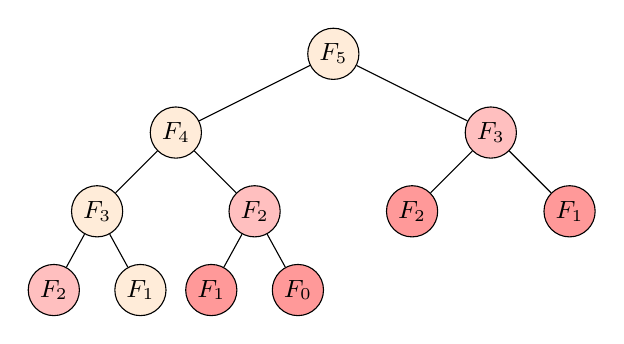
\begin{tikzpicture}[
    level distance=1cm,
    level 1/.style={sibling distance=4cm},
    level 2/.style={sibling distance=2cm},
    level 3/.style={sibling distance=1.1cm},
    every node/.style={circle, draw, fill=orange!15,
                       inner sep=1pt, minimum size=0.65cm, font=\small}
]
\node {$F_5$}
  child { node {$F_4$}
    child { node {$F_3$}
      child { node[fill=red!25] {$F_2$} }
      child { node {$F_1$} }
    }
    child { node[fill=red!25] {$F_2$}
      child { node[fill=red!40] {$F_1$} }
      child { node[fill=red!40] {$F_0$} }
    }
  }
  child { node[fill=red!25] {$F_3$}
    child { node[fill=red!40] {$F_2$} }
    child { node[fill=red!40] {$F_1$} }
  };
\end{tikzpicture}

\vspace{0.3em}
{\small \textcolor{keyred}{Les nœuds rouges sont recalculés plusieurs fois !}}
\end{center}

Complexité : \textbf{exponentielle} $O(2^n)$.

\subsubsection{Bottom-up DP : $\Theta(n)$}

\begin{algorithm}[H]
\caption{Bottom-Up-Fib($n$)}
\begin{algorithmic}[1]
\State $r[0] \leftarrow 1$;\; $r[1] \leftarrow 1$
\For{$i = 2$ \textbf{to} $n$}
  \State $r[i] \leftarrow r[i-1] + r[i-2]$
\EndFor
\State \Return $r[n]$
\end{algorithmic}
\end{algorithm}

\begin{center}
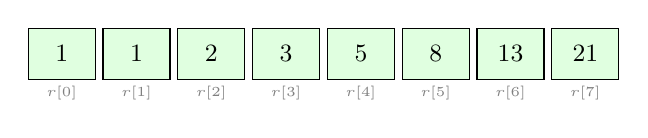
\begin{tikzpicture}[font=\small]
  \foreach \v/\i in {1/0, 1/1, 2/2, 3/3, 5/4, 8/5, 13/6, 21/7}{
    \node[draw, fill=green!12, minimum width=0.85cm, minimum height=0.65cm]
          at (\i*0.95, 0) {\v};
    \node[font=\tiny, gray] at (\i*0.95, -0.5) {$r[\i]$};
  }
\end{tikzpicture}
\end{center}

% ══════════════════════════════════════════════
\subsection{Coupe de tiges (\textit{Rod Cutting})}

\begin{definition}{Problème de la coupe de tiges}{rodcut}
\textbf{Entrée :} une tige de longueur $n$ et un tableau de prix $p_i$ pour une tige
de longueur $i$ ($1 \le i \le n$). \\
\textbf{Objectif :} trouver la découpe maximisant le revenu total.
\end{definition}

Il existe $2^{n-1}$ découpages possibles : la force brute est inenvisageable.

\subsubsection{Sous-structure optimale et récurrence}

\begin{theorem}{Structure optimale}{rodthm}
Si la première coupe optimale est après $i$ unités, et si
$s_1, \ldots, s_k$ est un découpage optimal de la tige restante de longueur $n-i$,
alors $i, s_1, \ldots, s_k$ est optimal pour la tige de longueur $n$.
\end{theorem}

Soit $r(n)$ le revenu optimal pour une tige de longueur $n$ :
\[
  r(n) =
  \begin{cases}
    0 & \text{si } n = 0, \\
    \displaystyle\max_{1 \le i \le n} \bigl\{ p_i + r(n-i) \bigr\} & \text{si } n \ge 1.
  \end{cases}
\]

\begin{center}
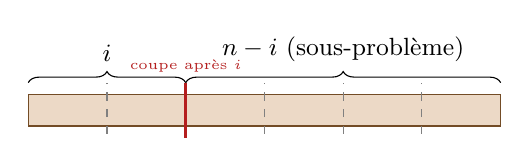
\begin{tikzpicture}[font=\small, >=Stealth]
  % Rod
  \draw[fill=brown!30, draw=brown!60!black] (0,-0.2) rectangle (6,0.2);
  \foreach \x in {1,2,3,4,5}{
    \draw[dashed, gray] (\x,-0.3) -- (\x,0.35);
  }
  \draw[keyred, very thick] (2,-0.35) -- (2,0.35)
        node[above, keyred, font=\tiny] {coupe après $i$};
  \draw[decorate, decoration={brace, amplitude=4pt}] (0,0.35) -- (2,0.35)
        node[midway, above=4pt] {$i$};
  \draw[decorate, decoration={brace, amplitude=4pt}] (2,0.35) -- (6,0.35)
        node[midway, above=4pt] {$n-i$ (sous-problème)};
\end{tikzpicture}
\end{center}

\begin{complexity}{DP pour la coupe de tiges}{rcplx}
\begin{itemize}[noitemsep]
  \item Top-down avec mémoïsation : $O(n^2)$ (graphe de sous-problèmes).
  \item Bottom-up : $O(n^2)$.
\end{itemize}
\end{complexity}

\subsubsection{Reconstruction de la solution}

On maintient un tableau $s[j]$ stockant la première coupe optimale pour $r(j)$.
Ensuite, on trace-back : couper $s[n]$, puis résoudre sur $n - s[n]$.

\[
\begin{array}{ccccccccc}
\toprule
i    & 0 & 1 & 2 & 3 & 4  & 5  & 6  & 7  & 8  \\
\midrule
r[i] & 0 & 1 & 5 & 8 & 10 & 13 & 17 & 18 & 22 \\
s[i] & 0 & 1 & 2 & 3 &  2 &  2 &  6 &  1 &  2 \\
\bottomrule
\end{array}
\]

% ══════════════════════════════════════════════
\subsection{Problème du rendu de monnaie}

\begin{definition}{Rendu de monnaie}{change}
\textbf{Entrée :} $n$ dénominations $0 < w_1 < \cdots < w_n$ et un montant cible $W$. \\
\textbf{Sortie :} nombre minimum de pièces pour atteindre exactement $W$.
\end{definition}

Récurrence DP :
\[
  c(w) =
  \begin{cases}
    0 & \text{si } w = 0, \\
    \displaystyle\min_{\substack{1 \le j \le n \\ w_j \le w}} \bigl\{1 + c(w - w_j)\bigr\}
       & \text{si } w \ge 1.
  \end{cases}
\]

\textbf{Exemple :} $w_1=1, w_2=2, w_3=5$, $W=8$.
Optimal : 1 pièce de chaque $\Rightarrow$ 3 pièces au total.

Remplissage bottom-up de $w=0$ à $W$ : complexité $O(nW)$.

% ══════════════════════════════════════════════
\subsection{Recette générale pour la PD}

\begin{tcolorbox}[colback=lightblue, colframe=keyblue,
                  title={\textbf{Étapes de conception d'un algorithme DP}},
                  fonttitle=\bfseries]
\begin{enumerate}
  \item \textbf{Identifier les choix et la sous-structure optimale} : un choix réduit
        le problème à de plus petits sous-problèmes, dont les solutions optimales
        composent la solution globale.
  \item \textbf{Écrire une récurrence} pour la valeur optimale en fonction des
        sous-problèmes.
  \item \textbf{Éviter les recalculs} via mémoïsation (top-down) ou remplissage
        de table (bottom-up).
  \item \textbf{(Optionnel) Reconstruire la solution} en stockant les choix dans une
        table auxiliaire et en remontant le tracé.
\end{enumerate}
\end{tcolorbox}

\begin{center}
\renewcommand{\arraystretch}{1.35}
\begin{tabular}{lcl}
\toprule
\textbf{Problème} & \textbf{Complexité} & \textbf{Taille de la table} \\
\midrule
Fibonacci         & $\Theta(n)$   & $n+1$ entrées \\
Coupe de tiges    & $O(n^2)$      & $n+1$ entrées \\
Rendu de monnaie  & $O(nW)$       & $W+1$ entrées \\
\bottomrule
\end{tabular}
\end{center}

\section{Lecture 9 : DP – rebuild and matrice chain}
% ══════════════════════════════════════════════════════════════════════════════
% Lecture 9 : Programmation Dynamique – Coupe de tiges (reconstruction)
%             et Multiplication de chaînes de matrices
% ══════════════════════════════════════════════════════════════════════════════

% ─────────────────────────────────────────────────────────────────────────────
\subsection{Rappel : éléments clés d'un algorithme DP}

La programmation dynamique repose sur deux propriétés fondamentales :

\begin{enumerate}
  \item \textbf{Sous-structure optimale} : une solution optimale s'obtient en faisant
        un \emph{choix}, ce qui laisse un ou plusieurs sous-problèmes à résoudre,
        et la solution optimale globale résout ces sous-problèmes de façon optimale.
  \item \textbf{Sous-problèmes répétés} : un algorithme récursif naïf recalcule les mêmes
        sous-problèmes de nombreuses fois.
        \begin{itemize}
          \item \textbf{Top-down avec mémoïsation} : résoudre récursivement en
                mémorisant chaque résultat dans une table.
          \item \textbf{Bottom-up} : trier les sous-problèmes et résoudre d'abord
                les plus petits ; ainsi, quand on résout un sous-problème, les
                sous-problèmes dont il dépend sont déjà calculés.
        \end{itemize}
\end{enumerate}

% ─────────────────────────────────────────────────────────────────────────────
\subsection{Coupe de tiges – Reconstruction de la solution optimale}

En Lecture~8, l'algorithme DP renvoyait uniquement le revenu optimal $r(n)$.
Il est souvent nécessaire de récupérer \emph{comment} obtenir ce revenu, c'est-à-dire
les longueurs des morceaux à couper.

\subsubsection{Algorithme étendu avec table des décisions}

L'idée est de maintenir une table auxiliaire $s[0\ldots n]$ : $s[j]$ stocke la longueur
du premier morceau coupé (la \emph{décision}) correspondant au revenu optimal $r[j]$.

\begin{algorithm}[H]
\caption{Extended-Bottom-Up-Cut-Rod($p$, $n$)}
\begin{algorithmic}[1]
\State Créer les tableaux $r[0\ldots n]$ et $s[0\ldots n]$
\State $r[0] \leftarrow 0$
\For{$j = 1$ \textbf{to} $n$}
    \State $q \leftarrow -\infty$
    \For{$i = 1$ \textbf{to} $j$}
        \If{$q < p[i] + r[j - i]$}
            \State $q \leftarrow p[i] + r[j - i]$  \AlgComment{meilleur revenu}
            \State $s[j] \leftarrow i$              \AlgComment{stocker le choix optimal}
        \EndIf
    \EndFor
    \State $r[j] \leftarrow q$
\EndFor
\State \Return $r$ et $s$
\end{algorithmic}
\end{algorithm}

La complexité reste $\Theta(n^2)$. La seule différence avec l'algorithme de base
est le maintien de $s[j]$ qui enregistre l'indice $i$ réalisant le maximum.

\subsubsection{Exemple : tables $r$ et $s$ pour $n = 8$}

En utilisant la table de prix $p_i$ : 1, 5, 8, 9, 10, 17, 17, 20, 24, 30 :

\begin{center}
\renewcommand{\arraystretch}{1.3}
\begin{tabular}{ccccccccccc}
\toprule
$i$    & 0 & 1 & 2 & 3 & 4  & 5  & 6  & 7  & 8  \\
\midrule
$r[i]$ & 0 & 1 & 5 & 8 & 10 & 13 & 17 & 18 & 22 \\
$s[i]$ & 0 & 1 & 2 & 3 & 2  & 2  & 6  & 1  & 2  \\
\bottomrule
\end{tabular}
\end{center}

\subsubsection{Extraction de la solution}

La table $s$ stocke les choix menant à une solution optimale.
On remonte la solution en traçant-back depuis $n$ :

\begin{algorithm}[H]
\caption{Print-Cut-Rod-Solution($p$, $n$)}
\begin{algorithmic}[1]
\State $(r, s) \leftarrow \textsc{Extended-Bottom-Up-Cut-Rod}(p, n)$
\While{$n > 0$}
    \State \textbf{afficher} $s[n]$   \AlgComment{taille du prochain morceau}
    \State $n \leftarrow n - s[n]$
\EndWhile
\end{algorithmic}
\end{algorithm}

\textbf{Trace pour $n = 8$ :}

\begin{center}
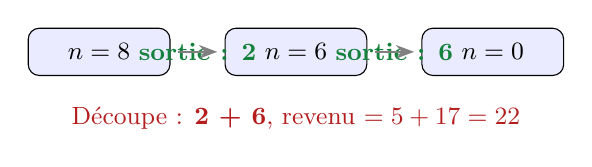
\begin{tikzpicture}[font=\small, >=Stealth]
  \foreach \n/\out/\x in {8/{}/0, 6/{2}/2.5, 0/{6}/5}{
    \node[draw, fill=blue!8, rounded corners, minimum width=1.8cm,
          minimum height=0.6cm, align=center] at (\x, 0) {$n = \n$};
    \ifx\out\empty\else
      \node[draw=none, fill=none, keygreen, font=\bfseries\small] at (\x-1.25, 0)
            {sortie : \out};
    \fi
  }
  \draw[->, thick, gray] (1.0, 0) -- (1.5, 0);
  \draw[->, thick, gray] (3.5, 0) -- (4.0, 0);
  \node[below=8pt, keyred, font=\small] at (2.5, -0.3)
        {Découpe : \textbf{2 + 6}, revenu $= 5 + 17 = 22$};
\end{tikzpicture}
\end{center}

% ─────────────────────────────────────────────────────────────────────────────
\subsection{Résumé : coupe de tiges}

\begin{tcolorbox}[colback=lightblue, colframe=keyblue, fonttitle=\bfseries,
                  title={Récapitulatif DP – Coupe de tiges}]
\begin{itemize}[noitemsep]
  \item \textbf{Choix} : où effectuer la coupe la plus à gauche.
  \item \textbf{Sous-structure optimale} : le reste doit être découpé de façon optimale.
  \item \textbf{Récurrence} :
    \[
      r(n) =
      \begin{cases}
        0 & \text{si } n = 0, \\
        \displaystyle\max_{1 \le i \le n} \bigl\{p_i + r(n-i)\bigr\} & \text{si } n \ge 1.
      \end{cases}
    \]
  \item \textbf{Complexité} : $\Theta(n^2)$ (top-down ou bottom-up).
  \item \textbf{Reconstruction} : table auxiliaire $s$ + trace-back en $O(n)$.
\end{itemize}
\end{tcolorbox}

% ─────────────────────────────────────────────────────────────────────────────
\subsection{Quand peut-on utiliser la programmation dynamique ?}

\begin{enumerate}
  \item \textbf{Sous-structure optimale.}
    \begin{itemize}
      \item Une solution optimale peut être construite en combinant des solutions
            optimales de sous-problèmes.
      \item Cela implique que la valeur optimale peut être exprimée par une
            \emph{formule récursive}.
    \end{itemize}
  \item \textbf{Sous-problèmes répétés.}
    \begin{itemize}
      \item Un algorithme récursif naïf peut revisiter le même sous-problème
            de nombreuses fois.
    \end{itemize}
\end{enumerate}

\begin{remark}{Problème du rendu de monnaie}{change9}
La DP s'applique directement à ce problème classique. Avec $n$ dénominations
$0 < w_1 < \cdots < w_n$ et un montant cible $W$, on minimise le nombre de pièces :
\[
  \min\left\{\sum_{j=1}^{n} x_j \;:\; \sum_{j=1}^{n} w_j x_j = W,\; x_j \in \mathbb{Z}_{\ge 0}\right\}.
\]
\textbf{Exemple :} $w_1=1$, $w_2=2$, $w_3=5$, $W=8$.
Optimal : $x_1 = x_2 = x_3 = 1 \Rightarrow$ 3~pièces.
\end{remark}

% ══════════════════════════════════════════════════════════════════════════════
\section*{Multiplication de chaînes de matrices}
\addcontentsline{toc}{subsection}{Multiplication de chaînes de matrices}
% ══════════════════════════════════════════════════════════════════════════════

% ─────────────────────────────────────────────────────────────────────────────
\subsection{Coût de la multiplication de deux matrices}

Multiplier une matrice $A_{p \times q}$ par une matrice $B_{q \times r}$ produit une
matrice $C_{p \times r}$.

\begin{center}
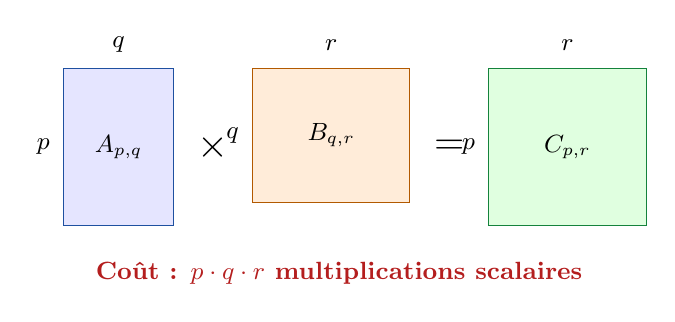
\begin{tikzpicture}[font=\small, >=Stealth]
  % Matrix A
  \draw[fill=blue!10, draw=keyblue] (0,0) rectangle (1.4, 2.0);
  \node at (0.7, 2.3) {$q$};
  \node[left] at (-0.05, 1.0) {$p$};
  \node at (0.7, 1.0) {$A_{p,q}$};
  \node[font=\Large] at (1.9, 1.0) {$\times$};
  % Matrix B
  \draw[fill=orange!15, draw=orange!70!black] (2.4,0.3) rectangle (4.4, 2.0);
  \node at (3.4, 2.3) {$r$};
  \node[left] at (2.35, 1.15) {$q$};
  \node at (3.4, 1.15) {$B_{q,r}$};
  \node[font=\Large] at (4.9, 1.0) {$=$};
  % Matrix C
  \draw[fill=green!12, draw=keygreen] (5.4, 0) rectangle (7.4, 2.0);
  \node at (6.4, 2.3) {$r$};
  \node[left] at (5.35, 1.0) {$p$};
  \node at (6.4, 1.0) {$C_{p,r}$};
  % Annotation
  \node[below=4pt, keyred, font=\bfseries\small] at (3.5, -0.2)
        {Coût : $p \cdot q \cdot r$ multiplications scalaires};
\end{tikzpicture}
\end{center}

Chaque entrée de $C$ nécessite $q$ multiplications scalaires.
La matrice $C$ contient $p \cdot r$ entrées, donc le coût total est
$\mathbf{p \cdot q \cdot r}$ \textbf{multiplications scalaires}.

\begin{tcolorbox}[colback=lightyellow, colframe=orange!70!black, fonttitle=\bfseries,
                  title={Pourquoi l'ordre d'association importe-t-il ?}]
Pour $A$ ($20 \times 1$), $B$ ($1 \times 10$), $C$ ($10 \times 100$) :
\begin{itemize}[noitemsep]
  \item $(A \times (B \times C))$ : $1\cdot10\cdot100 + 20\cdot1\cdot100 = 3\,000$
  \item $((A \times B) \times C)$ : $20\cdot1\cdot10 + 20\cdot10\cdot100 = 20\,200$
\end{itemize}
La parenthésisation peut \textbf{modifier radicalement} le nombre d'opérations.
\end{tcolorbox}

% ─────────────────────────────────────────────────────────────────────────────
\subsection{Définition du problème}

\begin{definition}{Multiplication de chaînes de matrices}{mcm}
\textbf{Entrée :} une chaîne $\langle A_1, A_2, \ldots, A_n \rangle$ de $n$ matrices,
où la matrice $A_i$ a la dimension $p_{i-1} \times p_i$ pour $i = 1, \ldots, n$.

\textbf{Sortie :} une parenthésisation complète du produit $A_1 A_2 \cdots A_n$
minimisant le nombre de multiplications scalaires.
\end{definition}

\textbf{Remarques :}
\begin{itemize}
  \item On ne demande \emph{pas} de calculer le produit, seulement de trouver la
        meilleure parenthésisation.
  \item La parenthésisation peut affecter considérablement le nombre de
        multiplications.
\end{itemize}

\textbf{Exemple :} chaîne $A_1 A_2 A_3$ avec dimensions $50\times5$, $5\times100$,
$100\times10$ :

\begin{center}
\renewcommand{\arraystretch}{1.3}
\begin{tabular}{lrl}
\toprule
\textbf{Parenthésisation} & \textbf{Coût} & \textbf{Calcul} \\
\midrule
$(A_1 A_2) A_3$ & $75\,000$ & $50\cdot5\cdot100 + 50\cdot100\cdot10$ \\
$A_1 (A_2 A_3)$ & $7\,500$  & $5\cdot100\cdot10 + 50\cdot5\cdot10$ \\
\bottomrule
\end{tabular}
\end{center}

% ─────────────────────────────────────────────────────────────────────────────
\subsection{Sous-structure optimale}

\begin{theorem}{Sous-structure optimale – Multiplication de matrices}{mcmopt}
Supposons que la parenthésisation optimale de $A_1 A_2 \cdots A_n$ effectue la
dernière multiplication comme $(A_1 \cdots A_k)(A_{k+1} \cdots A_n)$. Alors les
parenthésisations de $A_1 \cdots A_k$ et $A_{k+1} \cdots A_n$ dans cette solution
optimale sont elles-mêmes optimales.
\end{theorem}

\begin{proof}
Soit $M(P)$ le nombre de multiplications scalaires d'une parenthésisation $P$.
Notons $((O_L) \cdot (O_R))$ la solution optimale où $O_L$ et $O_R$ parenthésisent
respectivement $A_1\cdots A_k$ et $A_{k+1}\cdots A_n$. Soient $P_L$ et $P_R$ des
parenthésisations optimales de ces deux sous-chaînes. On a :
\begin{align*}
  M((O_L) \cdot (O_R))
    &= p_0 \cdot p_k \cdot p_n + M(O_L) + M(O_R) \\
    &\ge p_0 \cdot p_k \cdot p_n + M(P_L) + M(P_R)
     = M((P_L) \cdot (P_R)).
\end{align*}
Puisque $((O_L)\cdot(O_R))$ est optimal, on a l'égalité, donc
$M(P_L) = M(O_L)$ et $M(P_R) = M(O_R)$ : $P_L$ et $P_R$ sont bien optimales.
\end{proof}

% ─────────────────────────────────────────────────────────────────────────────
\subsection{Formule récursive}

Soit $m[i, j]$ le nombre minimal de multiplications scalaires pour calculer
$A_i A_{i+1} \cdots A_j$.

\[
  m[i, j] =
  \begin{cases}
    0 & \text{si } i = j, \\
    \displaystyle\min_{i \le k < j}
      \bigl\{ m[i,k] + m[k+1,j] + p_{i-1}\, p_k\, p_j \bigr\}
    & \text{si } i < j.
  \end{cases}
\]

\begin{remark}{Ordre de remplissage}{ordrem}
$m[i, j]$ ne dépend que de sous-problèmes avec un intervalle $j - i$ \emph{plus petit}.
Un algorithme bottom-up résout donc les sous-problèmes par ordre croissant de $j - i$
(longueur de chaîne $\ell = j - i + 1$).
\end{remark}

% ─────────────────────────────────────────────────────────────────────────────
\subsection{Algorithme bottom-up}

\begin{algorithm}[H]
\caption{Matrix-Chain-Order($p$)}
\begin{algorithmic}[1]
\State $n \leftarrow p.\mathit{length} - 1$
\State Créer les tables $m[1\ldots n,\, 1\ldots n]$ et $s[1\ldots n,\, 1\ldots n]$
\For{$i = 1$ \textbf{to} $n$}
    \State $m[i, i] \leftarrow 0$
\EndFor
\For{$\ell = 2$ \textbf{to} $n$}                  \AlgComment{$\ell$ = longueur de la chaîne}
    \For{$i = 1$ \textbf{to} $n - \ell + 1$}
        \State $j \leftarrow i + \ell - 1$
        \State $m[i, j] \leftarrow \infty$
        \For{$k = i$ \textbf{to} $j - 1$}
            \State $q \leftarrow m[i,k] + m[k+1,j] + p_{i-1}\, p_k\, p_j$
            \If{$q < m[i,j]$}
                \State $m[i,j] \leftarrow q$
                \State $s[i,j] \leftarrow k$   \AlgComment{$s$ mémorise le choix optimal}
            \EndIf
        \EndFor
    \EndFor
\EndFor
\State \Return $m$ et $s$
\end{algorithmic}
\end{algorithm}

\begin{complexity}{Matrix-Chain-Order}{mcmcplx}
\begin{itemize}[noitemsep]
  \item La table $m$ contient $O(n^2)$ entrées.
  \item Chaque entrée $m[i,j]$ requiert $O(n)$ pour trouver le meilleur $k$.
  \item \textbf{Complexité totale : $\Theta(n^3)$ en temps, $\Theta(n^2)$ en espace.}
\end{itemize}
\end{complexity}

% ─────────────────────────────────────────────────────────────────────────────
\subsection{Exemple complet}

Chaîne de $n = 6$ matrices avec dimensions :

\begin{center}
\renewcommand{\arraystretch}{1.2}
\begin{tabular}{lcccccc}
\toprule
Matrice     & $A_1$          & $A_2$          & $A_3$         & $A_4$        & $A_5$          & $A_6$ \\
\midrule
Dimensions & $30\times35$ & $35\times15$ & $15\times5$ & $5\times10$ & $10\times20$ & $20\times25$ \\
\bottomrule
\end{tabular}
\end{center}

\noindent Soit $p = \langle 30, 35, 15, 5, 10, 20, 25 \rangle$.

Les tables $m$ (coûts optimaux) et $s$ (choix optimaux) calculées par
\textsc{Matrix-Chain-Order} sont :

\begin{center}
\renewcommand{\arraystretch}{1.4}
\begin{tabular}{c|cccccc}
\multicolumn{7}{c}{\textbf{Table $m[i,j]$}} \\
\hline
$j \backslash i$ & 1 & 2 & 3 & 4 & 5 & 6 \\
\hline
1 & 0 & & & & & \\
2 & 15\,750 & 0 & & & & \\
3 & 7\,875 & 2\,625 & 0 & & & \\
4 & 9\,375 & 4\,375 & 750 & 0 & & \\
5 & 11\,875 & 7\,125 & 2\,500 & 1\,000 & 0 & \\
6 & 15\,125 & 10\,500 & 5\,375 & 3\,500 & 5\,000 & 0 \\
\hline
\end{tabular}
\qquad
\begin{tabular}{c|cccccc}
\multicolumn{7}{c}{\textbf{Table $s[i,j]$}} \\
\hline
$j \backslash i$ & 1 & 2 & 3 & 4 & 5 & 6 \\
\hline
2 & 1 & & & & & \\
3 & 1 & 2 & & & & \\
4 & 3 & 3 & 3 & & & \\
5 & 3 & 3 & 3 & 4 & & \\
6 & 3 & 3 & 3 & 5 & 5 & \\
\hline
\end{tabular}
\end{center}

La solution optimale est $m[1,6] = 15\,125$ multiplications scalaires.
En remontant depuis $s[1,6] = 3$, on obtient la parenthésisation :
\[
  \bigl(A_1 \,(A_2\,A_3)\bigr)\bigl((A_4\,A_5)\,A_6\bigr)
\]

% ─────────────────────────────────────────────────────────────────────────────
\subsection{Reconstruction de la parenthésisation optimale}

La table $s$ permet de reconstruire récursivement la parenthésisation :

\begin{algorithm}[H]
\caption{Print-Optimal-Parens($s$, $i$, $j$)}
\begin{algorithmic}[1]
\If{$i = j$}
    \State \textbf{afficher} ``$A_i$''
\Else
    \State \textbf{afficher} ``(''
    \State \Call{Print-Optimal-Parens}{$s$, $i$, $s[i,j]$}
    \State \Call{Print-Optimal-Parens}{$s$, $s[i,j]+1$, $j$}
    \State \textbf{afficher} ``)''
\EndIf
\end{algorithmic}
\end{algorithm}

\textbf{Trace pour l'exemple ($i=1$, $j=6$) :}

\begin{center}
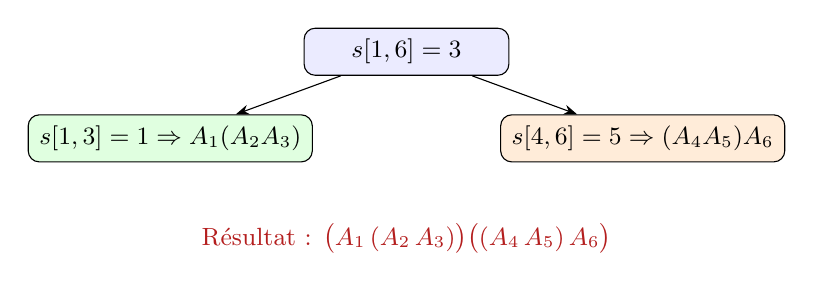
\begin{tikzpicture}[font=\small, >=Stealth,
    node/.style={draw, rounded corners, fill=blue!8,
                 minimum width=2.6cm, minimum height=0.55cm,
                 inner sep=4pt}]
  \node[node] (r) at (0, 0) {$s[1,6]=3$};
  \node[node, fill=green!12] (l) at (-3, -1.1) {$s[1,3]=1 \Rightarrow A_1(A_2 A_3)$};
  \node[node, fill=orange!15] (r2) at (3, -1.1) {$s[4,6]=5 \Rightarrow (A_4 A_5)A_6$};
  \draw[->] (r) -- (l);
  \draw[->] (r) -- (r2);
  \node[below=16pt, keyred] at (0, -1.5)
        {Résultat : $\bigl(A_1\,(A_2\,A_3)\bigr)\bigl((A_4\,A_5)\,A_6\bigr)$};
\end{tikzpicture}
\end{center}

% ─────────────────────────────────────────────────────────────────────────────
\subsection{Résumé : multiplication de chaînes de matrices}

\begin{tcolorbox}[colback=lightblue, colframe=keyblue, fonttitle=\bfseries,
                  title={Récapitulatif DP – Multiplication de chaînes de matrices}]
\begin{itemize}[noitemsep]
  \item \textbf{Choix} : où placer la parenthèse la plus externe
        $(A_1 \cdots A_k)(A_{k+1} \cdots A_n)$.
  \item \textbf{Sous-structure optimale} : les deux sous-chaînes doivent être
        parenthésées de façon optimale (prouvé par l'argument de cut-and-paste).
  \item \textbf{Récurrence} :
    \[
      m[i,j] =
      \begin{cases}
        0 & \text{si } i = j, \\
        \displaystyle\min_{i \le k < j}
          \bigl\{m[i,k] + m[k+1,j] + p_{i-1}\,p_k\,p_j\bigr\}
        & \text{si } i < j.
      \end{cases}
    \]
  \item \textbf{Complexité} : $\Theta(n^3)$ en temps, $\Theta(n^2)$ en espace.
  \item \textbf{Reconstruction} : table auxiliaire $s$ + \textsc{Print-Optimal-Parens}.
\end{itemize}
\end{tcolorbox}

% ─────────────────────────────────────────────────────────────────────────────
\subsection{Recette générale pour la DP (consolidation)}

\begin{center}
\renewcommand{\arraystretch}{1.45}
\begin{tabular}{llcl}
\toprule
\textbf{Problème} & \textbf{Choix} & \textbf{Complexité} & \textbf{Taille de la table} \\
\midrule
Coupe de tiges     & Position de la coupe gauche & $\Theta(n^2)$   & $n+1$ entrées \\
Rendu de monnaie   & Dénomination utilisée       & $O(nW)$         & $W+1$ entrées \\
Chaînes de matrices & Position de la parenthèse  & $\Theta(n^3)$   & $n^2$ entrées \\
\bottomrule
\end{tabular}
\end{center}

Les trois étapes systématiques restent :
\begin{enumerate}
  \item Identifier les choix et la sous-structure optimale.
  \item Écrire la récurrence pour la valeur optimale.
  \item Résoudre efficacement (top-down avec mémoïsation ou bottom-up).
\end{enumerate}

\section{Lecture 10 : DP – longest common subsequence}
% ══════════════════════════════════════════════════════════════════════════════
% Lecture 10: Dynamic Programming – Longest Common Subsequence (LCS)
% ══════════════════════════════════════════════════════════════════════════════

% ══════════════════════════════════════════════════════════════════════════════
\section*{Longest Common Subsequence (LCS)}
\addcontentsline{toc}{subsection}{Longest Common Subsequence (LCS)}
% ══════════════════════════════════════════════════════════════════════════════

% ─────────────────────────────────────────────────────────────────────────────
\subsection{Definition and Motivation}

\begin{definition}{Longest Common Subsequence}{lcs}
\textbf{Input:} two sequences $X = \langle x_1, \ldots, x_m \rangle$ and
$Y = \langle y_1, \ldots, y_n \rangle$.

\textbf{Output:} a common subsequence to both whose length is maximal.

\textbf{Reminder:} a subsequence does not need to be consecutive, but must
respect the order of the elements.
\end{definition}

\textbf{Example:} for the words \texttt{heroically} and \texttt{scholarly}, the LCS
is \texttt{holly} (length~5): the letters appear in the correct order in
each of the two words, without necessarily being adjacent.

% ─────────────────────────────────────────────────────────────────────────────
\subsection{Why Naive Approaches Fail}

\textbf{Brute force:} for each subsequence of $X$, check if it is
a subsequence of $Y$.

\begin{complexity}{Brute force for LCS}{lcsbf}
\begin{itemize}[noitemsep]
  \item $X$ has $2^m$ subsequences.
  \item Each verification takes $\Theta(n)$ (traversing $Y$ letter by letter).
  \item \textbf{Total complexity: $\Theta(n \cdot 2^m)$ — exponential, unusable.}
\end{itemize}
\end{complexity}

There is also no natural greedy algorithm for this problem:
the locally best letter does not necessarily lead to the global optimal
solution. Dynamic programming is the right tool.

% ─────────────────────────────────────────────────────────────────────────────
\subsection{Intuition of the DP Approach}

We traverse the two sequences from the \emph{right} (the end) to the left,
step by step.

At each position $(i, j)$ (looking at $x_i$ and $y_j$):
\begin{itemize}
  \item \textbf{If $x_i = y_j$}: this letter is part of the LCS; we include it
        and solve the subproblem on prefixes $X_{i-1}$ and $Y_{j-1}$.
  \item \textbf{If $x_i \ne y_j$}: the optimal LCS is obtained by moving one step
        to the left in \emph{one} of the two sequences, and taking the best of the
        two results.
\end{itemize}

\begin{center}
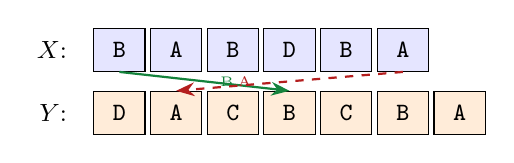
\begin{tikzpicture}[font=\small, >=Stealth]
  % X sequence
  \foreach \c/\i in {B/0,A/1,B/2,D/3,B/4,A/5}{
    \node[draw, fill=blue!10, minimum width=0.65cm, minimum height=0.55cm]
          at (\i*0.72, 0.8) {\texttt{\c}};
  }
  \node[left=4pt] at (-0.4, 0.8) {$X$:};
  % Y sequence
  \foreach \c/\i in {D/0,A/1,C/2,B/3,C/4,B/5,A/6}{
    \node[draw, fill=orange!15, minimum width=0.65cm, minimum height=0.55cm]
          at (\i*0.72, 0) {\texttt{\c}};
  }
  \node[left=4pt] at (-0.4, 0) {$Y$:};
  % Arrows for matching letters
  \draw[->, keygreen, thick] (0*0.72, 0.52) -- (3*0.72, 0.28)
        node[midway, right=2pt, font=\tiny, keygreen]{B};
  \draw[->, keyred, thick, dashed] (5*0.72, 0.52) -- (1*0.72, 0.28)
        node[midway, left=10pt, font=\tiny, keyred]{A};
\end{tikzpicture}
\end{center}

% ─────────────────────────────────────────────────────────────────────────────
\subsection{Optimal Substructure}

Let $X_i = \langle x_1, x_2, \ldots, x_i \rangle$ and
$Y_j = \langle y_1, y_2, \ldots, y_j \rangle$ be the prefixes of length $i$ and $j$.

\begin{theorem}{Optimal Substructure for LCS}{lcsopt}
Let $Z = \langle z_1, z_2, \ldots, z_k \rangle$ be an LCS of $X_i$ and $Y_j$.
\begin{enumerate}
  \item \textbf{If $x_i = y_j$}: then $z_k = x_i = y_j$ and $Z_{k-1}$ is an
        LCS of $X_{i-1}$ and $Y_{j-1}$.
  \item \textbf{If $x_i \ne y_j$ and $z_k \ne x_i$}: then $Z$ is an LCS of
        $X_{i-1}$ and $Y_j$.
  \item \textbf{If $x_i \ne y_j$ and $z_k \ne y_j$}: then $Z$ is an LCS of
        $X_i$ and $Y_{j-1}$.
\end{enumerate}
\end{theorem}

\begin{proof}
\textbf{Case 1 ($x_i = y_j$).}
If $z_k \ne x_i = y_j$, then $Z' = \langle z_1, \ldots, z_k, x_i \rangle$ is a
common subsequence of $X_i$ and $Y_j$ of length $k+1$, which contradicts
the optimality of $Z$. Thus $z_k = x_i = y_j$.

Now suppose that $Z_{k-1}$ is not an LCS of $X_{i-1}$ and $Y_{j-1}$:
there would exist a common subsequence $W$ of $X_{i-1}$ and $Y_{j-1}$ of
length $\ge k$. Then $\langle W, z_k \rangle$ would be a common subsequence
of $X_i$ and $Y_j$ of length $\ge k+1$, a contradiction.

\textbf{Case 2 ($x_i \ne y_j$, $z_k \ne x_i$).}
$Z$ is already a common subsequence of $X_{i-1}$ and $Y_j$. If it were not
optimal, there would exist $W$ of length $> k$ as a subsequence of $X_{i-1}$ and $Y_j$,
which would also be a subsequence of $X_i$ and $Y_j$ (since $W$ does not end with $x_i$),
contradicting the optimality of $Z$. Case~3 is symmetric.
\end{proof}

% ─────────────────────────────────────────────────────────────────────────────
\subsection{Recursive Formulation}

It follows from the previous theorem that the length of the LCS of $X_i$ and $Y_j$ is:

\[
  c[i, j] = \text{length of the LCS of } X_i \text{ and } Y_j
\]

with the recurrence:

\[
  c[i, j] =
  \begin{cases}
    0 & \text{if } i = 0 \text{ or } j = 0, \\
    c[i-1, j-1] + 1 & \text{if } i, j > 0 \text{ and } x_i = y_j, \\
    \max\bigl(c[i-1, j],\; c[i, j-1]\bigr) & \text{if } i, j > 0 \text{ and } x_i \ne y_j.
  \end{cases}
\]

We want to compute $c[m, n]$.

\begin{remark}{Overlapping Subproblems}{lcsov}
A naive recursion would solve the same subproblems an exponential number of times.
The bottom-up approach fills the table $c$ only once, by processing the
subproblems by increasing size (rows $i$ from $0$ to $m$, columns $j$ from $0$ to $n$).
\end{remark}

% ─────────────────────────────────────────────────────────────────────────────
\subsection{Bottom-up Algorithm and Complete Example}

For $X = \langle B,A,B,D,B,A \rangle$ and $Y = \langle D,A,C,B,C,B,A \rangle$
($m = 6$, $n = 7$), here is the complete table $c[i,j]$:

\begin{center}
\renewcommand{\arraystretch}{1.4}
\begin{tabular}{|c|c|c|c|c|c|c|c|c|c|}
& & \multicolumn{7}{c}{$j$} \\
$i$ & & \textbf{0} & \textbf{1 (D)} & \textbf{2 (A)} & \textbf{3 (C)} &
          \textbf{4 (B)} & \textbf{5 (C)} & \textbf{6 (B)} & \textbf{7 (A)} \\
\hline
\textbf{0}      & & 0 & 0 & 0 & 0 & 0 & 0 & 0 & 0 \\
\textbf{1 (B)}  & & 0 & 0 & 0 & 0 & 1 & 1 & 1 & 1 \\
\textbf{2 (A)}  & & 0 & 0 & 1 & 1 & 1 & 1 & 1 & 2 \\
\textbf{3 (B)}  & & 0 & 0 & 1 & 1 & 2 & 2 & 2 & 2 \\
\textbf{4 (D)}  & & 0 & 1 & 1 & 1 & 2 & 2 & 2 & 2 \\
\textbf{5 (B)}  & & 0 & 1 & 1 & 1 & 2 & 2 & 3 & 3 \\
\textbf{6 (A)}  & & 0 & 1 & 2 & 2 & 2 & 2 & 3 & \cellcolor{blue!20}\textbf{4} \\
\end{tabular}
\end{center}

The LCS has length \textbf{4} (value $c[6,7]$). By tracing back the decisions, we
obtain the LCS \textbf{ABBA}.

\begin{remark}{Reading the Table}{lcstable}
To fill $c[i,j]$: if $x_i = y_j$, come from the diagonal ($c[i-1,j-1]+1$).
Otherwise, take the maximum of the cell above ($c[i-1,j]$) and the cell
to the left ($c[i,j-1]$).
\end{remark}

% ─────────────────────────────────────────────────────────────────────────────
\subsection{Pseudocode}

\begin{algorithm}[H]
\caption{LCS-Length($X$, $Y$)}
\begin{algorithmic}[1]
\State $m \leftarrow X.\mathit{length}$;\; $n \leftarrow Y.\mathit{length}$
\State Create tables $c[0\ldots m,\; 0\ldots n]$ and $b[1\ldots m,\; 1\ldots n]$
\For{$i = 0$ \textbf{to} $m$}
    \State $c[i, 0] \leftarrow 0$
\EndFor
\For{$j = 0$ \textbf{to} $n$}
    \State $c[0, j] \leftarrow 0$
\EndFor
\For{$i = 1$ \textbf{to} $m$}
    \For{$j = 1$ \textbf{to} $n$}
        \If{$x_i = y_j$}
            \State $c[i, j] \leftarrow c[i-1, j-1] + 1$
            \State $b[i, j] \leftarrow \text{``}\nwarrow\text{''}$   \AlgComment{diagonal: common letter}
        \ElsIf{$c[i-1, j] \ge c[i, j-1]$}
            \State $c[i, j] \leftarrow c[i-1, j]$
            \State $b[i, j] \leftarrow \text{``}\uparrow\text{''}$   \AlgComment{up: advance in $X$}
        \Else
            \State $c[i, j] \leftarrow c[i, j-1]$
            \State $b[i, j] \leftarrow \text{``}\leftarrow\text{''}$ \AlgComment{left: advance in $Y$}
        \EndIf
    \EndFor
\EndFor
\State \Return $c$ and $b$
\end{algorithmic}
\end{algorithm}

\begin{complexity}{LCS-Length}{lcscplx}
\begin{itemize}[noitemsep]
  \item Table $c$ contains $(m+1)(n+1)$ entries, each calculated in $\Theta(1)$.
  \item \textbf{Time complexity: $\Theta(m \cdot n)$.}
  \item \textbf{Space complexity: $\Theta(m \cdot n)$.}
\end{itemize}
\end{complexity}

% ─────────────────────────────────────────────────────────────────────────────
\subsection{LCS Reconstruction}

Table $b$ stores the optimal choices: we trace it back recursively from
$b[m, n]$ toward the upper-left corner.

\begin{algorithm}[H]
\caption{Print-LCS($b$, $X$, $i$, $j$)}
\begin{algorithmic}[1]
\If{$i = 0$ \textbf{or} $j = 0$}
    \State \Return
\EndIf
\If{$b[i, j] = \text{``}\nwarrow\text{''}$}
    \State \Call{Print-LCS}{$b$, $X$, $i-1$, $j-1$}
    \State \textbf{print} $x_i$         \AlgComment{common letter: we include it}
\ElsIf{$b[i, j] = \text{``}\uparrow\text{''}$}
    \State \Call{Print-LCS}{$b$, $X$, $i-1$, $j$}
\Else
    \State \Call{Print-LCS}{$b$, $X$, $i$, $j-1$}
\EndIf
\end{algorithmic}
\end{algorithm}

\begin{complexity}{Print-LCS}{printlcscplx}
\begin{itemize}[noitemsep]
  \item Each recursive call decreases $i + j$ by at least 1.
  \item The recurrence satisfies $T(n) \le T(n-1) + \Theta(1)$, hence $T(n) = O(n)$.
  \item \textbf{Total complexity: $\Theta(|X| + |Y|)$}
        (the lower bound comes from $T(n) \ge T(n-2) + \Theta(1)$).
\end{itemize}
\end{complexity}

% ─────────────────────────────────────────────────────────────────────────────
\subsection{Backtracking Illustration}

For $X = \langle B,A,B,D,B,A \rangle$, $Y = \langle D,A,C,B,C,B,A \rangle$,
the path in table $b$ (illustrated below) identifies the letters \textbf{A, B, B, A}
= \textbf{ABBA} as the LCS:

\begin{center}
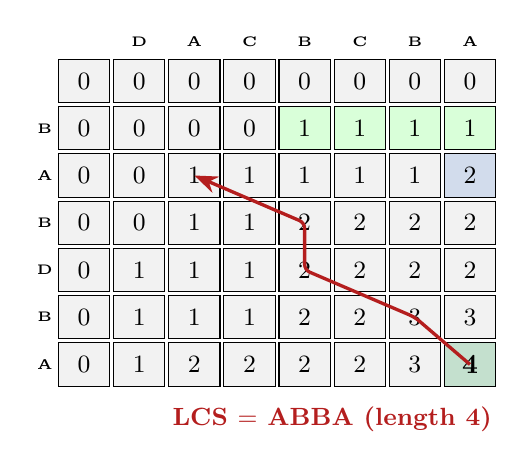
\begin{tikzpicture}[font=\small, >=Stealth,
    cell/.style={draw, minimum width=0.65cm, minimum height=0.55cm, inner sep=1pt}]

  % Column headers (Y)
  \foreach \c/\j in {{}/0, D/1, A/2, C/3, B/4, C/5, B/6, A/7}{
    \node[font=\bfseries\tiny] at (\j*0.7+0.35, 4.5) {\c};
  }
  % Row headers (X)
  \foreach \c/\i in {{}/0, B/1, A/2, B/3, D/4, B/5, A/6}{
    \node[font=\bfseries\tiny] at (-0.15, 4.0-\i*0.6) {\c};
  }

  % Fill the table with values and arrows
  % Row 0
  \foreach \j in {0,...,7}{
    \node[cell, fill=gray!10] at (\j*0.7+0.35, 4.0) {0};
  }
  % Row 1: 0 0 0 0 1 1 1 1
  \foreach \v/\j in {0/0, 0/1, 0/2, 0/3, 1/4, 1/5, 1/6, 1/7}{
    \pgfmathparse{int(\v)}
    \ifnum\pgfmathresult=1
      \node[cell, fill=green!15] at (\j*0.7+0.35, 3.4) {\v};
    \else
      \node[cell, fill=gray!10] at (\j*0.7+0.35, 3.4) {\v};
    \fi
  }
  % Row 2: 0 0 1 1 1 1 1 2
  \foreach \v/\j in {0/0, 0/1, 1/2, 1/3, 1/4, 1/5, 1/6, 2/7}{
    \pgfmathparse{int(\v)}
    \ifnum\pgfmathresult=2
      \node[cell, fill=keyblue!20] at (\j*0.7+0.35, 2.8) {\v};
    \else
      \node[cell, fill=gray!10] at (\j*0.7+0.35, 2.8) {\v};
    \fi
  }
  % Row 3: 0 0 1 1 2 2 2 2
  \foreach \v/\j in {0/0, 0/1, 1/2, 1/3, 2/4, 2/5, 2/6, 2/7}{
    \node[cell, fill=gray!10] at (\j*0.7+0.35, 2.2) {\v};
  }
  % Row 4: 0 1 1 1 2 2 2 2
  \foreach \v/\j in {0/0, 1/1, 1/2, 1/3, 2/4, 2/5, 2/6, 2/7}{
    \node[cell, fill=gray!10] at (\j*0.7+0.35, 1.6) {\v};
  }
  % Row 5: 0 1 1 1 2 2 3 3
  \foreach \v/\j in {0/0, 1/1, 1/2, 1/3, 2/4, 2/5, 3/6, 3/7}{
    \node[cell, fill=gray!10] at (\j*0.7+0.35, 1.0) {\v};
  }
  % Row 6: 0 1 2 2 2 2 3 4
  \foreach \v/\j in {0/0, 1/1, 2/2, 2/3, 2/4, 2/5, 3/6, 4/7}{
    \pgfmathparse{int(\v)}
    \ifnum\pgfmathresult=4
      \node[cell, fill=keygreen!25, font=\bfseries] at (\j*0.7+0.35, 0.4) {\v};
    \else
      \node[cell, fill=gray!10] at (\j*0.7+0.35, 0.4) {\v};
    \fi
  }

  % Traceback path arrows
  \draw[->, keyred, very thick, rounded corners=2pt]
    (7*0.7+0.35, 0.4)  % (6,7)=4, diagonal A match
    -- (6*0.7+0.35, 1.0)    % (5,6)=3, diagonal B match
    -- (4*0.7+0.35, 1.6)    % (4,4) up
    -- (4*0.7+0.35, 2.2)    % (3,4) diagonal B match
    -- (2*0.7+0.35, 2.8);   % (2,2) diagonal A match

  % Legend
  \node[keyred, font=\bfseries\small] at (3.5, -0.3)
        {LCS $=$ \textbf{ABBA} (length 4)};
\end{tikzpicture}
\end{center}

% ─────────────────────────────────────────────────────────────────────────────
\subsection{Summary: LCS}

\begin{tcolorbox}[colback=lightblue, colframe=keyblue, fonttitle=\bfseries,
                  title={Summary DP – Longest Common Subsequence}]
\begin{itemize}[noitemsep]
  \item \textbf{Choice}: if $x_i = y_j$, include this letter; otherwise advance in
        $X$ or in $Y$ (take the best of the two).
  \item \textbf{Optimal substructure}: 3 cases depending on whether $x_i = y_j$ or not
        (theorem above).
  \item \textbf{Recurrence}:
    \[
      c[i,j] =
      \begin{cases}
        0 & i = 0 \text{ or } j = 0,\\
        c[i-1,j-1]+1 & x_i = y_j,\\
        \max(c[i-1,j],\,c[i,j-1]) & x_i \ne y_j.
      \end{cases}
    \]
  \item \textbf{Complexity}: $\Theta(mn)$ in time and space.
  \item \textbf{Reconstruction}: table $b$ + \textsc{Print-LCS} in $\Theta(|X|+|Y|)$.
\end{itemize}
\end{tcolorbox}

% ─────────────────────────────────────────────────────────────────────────────
\subsection{General Overview of Dynamic Programming}

\begin{tcolorbox}[colback=lightyellow, colframe=orange!70!black, fonttitle=\bfseries,
                  title={DP Recipe in Three Steps}]
\begin{enumerate}
  \item \textbf{Identify the choices and the optimal substructure.}
  \item \textbf{Write the optimal value as a recurrence on subproblems.}
  \item \textbf{Solve efficiently}: top-down with memoization or bottom-up
        (without recalculating the same subproblems).
\end{enumerate}
\end{tcolorbox}

\begin{center}
\renewcommand{\arraystretch}{1.45}
\begin{tabular}{llcc}
\toprule
\textbf{Problem} & \textbf{Choice} & \textbf{Complexity} & \textbf{Table} \\
\midrule
Rod Cutting         & Left cut position               & $\Theta(n^2)$  & $n+1$ \\
Coin Change         & Denomination used               & $O(nW)$        & $W+1$ \\
Matrix Chains       & Parenthesis position            & $\Theta(n^3)$  & $n^2$ \\
LCS                 & Include $x_i = y_j$ / advance   & $\Theta(mn)$   & $(m+1)(n+1)$ \\
\bottomrule
\end{tabular}
\end{center}

\section{Lecture 11 : DP – binary tree of optimal research}
% ══════════════════════════════════════════════════════════════════════════════
% Lecture 11 : Programmation Dynamique – Arbres Binaires de Recherche Optimaux
% ══════════════════════════════════════════════════════════════════════════════

% ══════════════════════════════════════════════════════════════════════════════
\section*{Arbres Binaires de Recherche Optimaux (OBST)}
\addcontentsline{toc}{subsection}{Arbres Binaires de Recherche Optimaux}
% ══════════════════════════════════════════════════════════════════════════════

% ─────────────────────────────────────────────────────────────────────────────
\subsection{Motivation}

Dans un moteur de recherche, certains termes sont recherchés bien plus souvent que
d'autres. Si l'on stocke les clés dans un ABR, l'ordre de recherche dépend de la
structure de l'arbre. Placer les clés les plus fréquentes près de la racine permet
de minimiser le coût moyen d'une recherche. Le problème de l'OBST formalise cette idée.

% ─────────────────────────────────────────────────────────────────────────────
\subsection{Définition du problème}

\begin{definition}{Arbre Binaire de Recherche Optimal}{obst}
\textbf{Entrée :} une séquence triée de $n$ clés distinctes
$K = \langle k_1 < k_2 < \cdots < k_n \rangle$, avec pour chaque $k_i$ une
probabilité de recherche $p_i > 0$ (avec $\sum_{i=1}^n p_i = 1$).

\textbf{Objectif :} construire un ABR $T$ sur ces clés qui minimise le coût
de recherche espéré :
\[
  E[\text{coût de recherche dans } T]
  = \sum_{i=1}^{n} (\depth_T(k_i) + 1)\, p_i
  = 1 + \sum_{i=1}^{n} \depth_T(k_i)\cdot p_i.
\]
\end{definition}

Le coût réel d'une recherche de $k_i$ vaut $\depth_T(k_i) + 1$ (nombre de nœuds
examinés, racine incluse).

% ─────────────────────────────────────────────────────────────────────────────
\subsection{Exemple motivant}

Avec $n = 5$ clés et les probabilités :

\begin{center}
\renewcommand{\arraystretch}{1.3}
\begin{tabular}{lccccc}
\toprule
$i$   & 1    & 2   & 3    & 4   & 5   \\
\midrule
$p_i$ & 0.25 & 0.2 & 0.05 & 0.2 & 0.3 \\
\bottomrule
\end{tabular}
\end{center}

\textbf{Arbre A} (racine $k_2$) :

\begin{center}
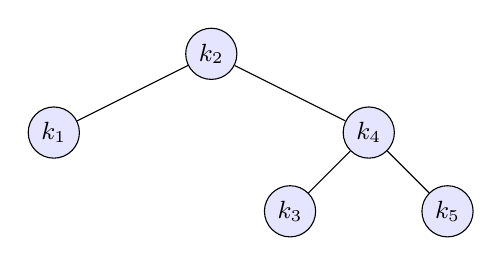
\begin{tikzpicture}[
    level distance=1.0cm,
    level 1/.style={sibling distance=4cm},
    level 2/.style={sibling distance=2cm},
    every node/.style={circle, draw, fill=blue!10,
                       inner sep=2pt, minimum size=0.65cm, font=\small}]
  \node {$k_2$}
    child { node {$k_1$} }
    child { node {$k_4$}
      child { node {$k_3$} }
      child { node {$k_5$} }
    };
\end{tikzpicture}
\end{center}

\begin{center}
\renewcommand{\arraystretch}{1.2}
\begin{tabular}{ccc}
\toprule
$i$ & $\depth_T(k_i)$ & $\depth_T(k_i) \cdot p_i$ \\
\midrule
1 & 1 & 0.25 \\
2 & 0 & 0    \\
3 & 2 & 0.10 \\
4 & 1 & 0.20 \\
5 & 2 & 0.60 \\
\midrule
  &   & $\sum = 1.15$ \\
\bottomrule
\end{tabular}
\end{center}

$E[\text{coût}] = 1 + 1.15 = 2.15$.

\textbf{Arbre B} (racine $k_2$, mais $k_5$ enfant droit de $k_2$, $k_4$ à gauche de $k_5$, $k_3$ à gauche de $k_4$) :

\begin{center}
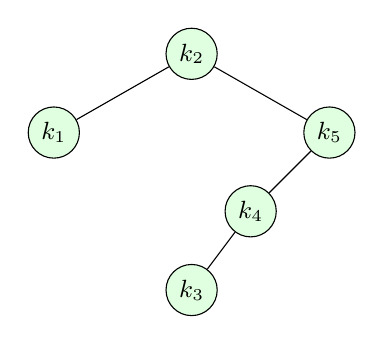
\begin{tikzpicture}[
    level distance=1.0cm,
    level 1/.style={sibling distance=3.5cm},
    level 2/.style={sibling distance=2cm},
    level 3/.style={sibling distance=1.5cm},
    every node/.style={circle, draw, fill=green!12,
                       inner sep=2pt, minimum size=0.65cm, font=\small}]
  \node {$k_2$}
    child { node {$k_1$} }
    child { node {$k_5$}
      child { node {$k_4$}
        child { node {$k_3$} }
        child[missing] {}
      }
      child[missing] {}
    };
\end{tikzpicture}
\end{center}

\begin{center}
\renewcommand{\arraystretch}{1.2}
\begin{tabular}{ccc}
\toprule
$i$ & $\depth_T(k_i)$ & $\depth_T(k_i) \cdot p_i$ \\
\midrule
1 & 1 & 0.25 \\
2 & 0 & 0    \\
3 & 3 & 0.15 \\
4 & 2 & 0.40 \\
5 & 1 & 0.30 \\
\midrule
  &   & $\sum = 1.10$ \\
\bottomrule
\end{tabular}
\end{center}

$E[\text{coût}] = 1 + 1.10 = \mathbf{2.10}$ — cet arbre s'avère être optimal.

\begin{remark}{Observations clés}{obsobs}
\begin{itemize}[noitemsep]
  \item L'OBST n'est \emph{pas} nécessairement l'arbre de hauteur minimale.
  \item La clé de plus grande probabilité n'est \emph{pas} nécessairement à la racine.
  \item Le nombre d'ABR à $n$ nœuds est exponentiel (nombres de Catalan $\sim 4^n/n^{3/2}$),
        donc la force brute est impraticable.
\end{itemize}
\end{remark}

% ─────────────────────────────────────────────────────────────────────────────
\subsection{Sous-structure optimale}

Un ABR se construit en choisissant une racine $k_r$, puis en construisant
récursivement le sous-arbre gauche sur $k_i, \ldots, k_{r-1}$ et le sous-arbre
droit sur $k_{r+1}, \ldots, k_j$.

\begin{theorem}{Sous-structure optimale de l'OBST}{obstopt}
Si l'on construit un ABT optimal sur $k_i, \ldots, k_j$ avec racine $k_r$, alors
les sous-arbres gauche et droit doivent eux aussi être des OBST (sur
$k_i, \ldots, k_{r-1}$ et $k_{r+1}, \ldots, k_j$ respectivement).
\end{theorem}

\textbf{Analyse du coût.} En notant $w(i,j) = \sum_{\ell=i}^{j} p_\ell$ la somme
des probabilités sur $k_i, \ldots, k_j$, on observe que quand un sous-arbre devient
le fils gauche ou droit de la racine, la profondeur de chacun de ses nœuds augmente
de~1. Donc :

\[
  E[\text{coût sous-arbre } k_i \ldots k_j]
  = p_r + \bigl(w(i,r-1) + E[\text{coût gauche}]\bigr)
        + \bigl(w(r+1,j) + E[\text{coût droit}]\bigr).
\]

En regroupant, on obtient :
\[
  E[\text{coût}] = p_r + w(i,r-1) + E[\text{coût gauche}] + w(r+1,j) + E[\text{coût droit}]
                 = w(i,j) + E[\text{coût gauche}] + E[\text{coût droit}].
\]

% ─────────────────────────────────────────────────────────────────────────────
\subsection{Formulation récursive}

Définissons $e[i,j]$ comme le coût de recherche espéré de l'OBST construit sur
$k_i, \ldots, k_j$, et $w(i,j) = \sum_{\ell=i}^{j} p_\ell$.

\[
  e[i, j] =
  \begin{cases}
    0 & \text{si } i = j + 1 \quad (\text{sous-arbre vide}), \\[6pt]
    \displaystyle\min_{i \le r \le j}
      \bigl\{ e[i, r-1] + e[r+1, j] + w(i,j) \bigr\}
    & \text{si } i \le j.
  \end{cases}
\]

On veut calculer $e[1, n]$.

\begin{remark}{Lien avec la somme des probabilités}{wlink}
Le terme $w(i,j) = \sum_{\ell=i}^{j} p_\ell$ peut être précalculé de façon
incrémentale : $w(i,j) = w(i,j-1) + p_j$, ce qui évite de le recalculer à chaque
étape.
\end{remark}

% ─────────────────────────────────────────────────────────────────────────────
\subsection{Algorithme bottom-up}

On remplit les tables $e$ et $r$ (racines optimales) par longueur de chaîne
croissante ($\ell = j - i + 1$ de 1 à $n$) :

\begin{algorithm}[H]
\caption{Optimal-BST($p$, $n$)}
\begin{algorithmic}[1]
\State Créer les tables $e[1\ldots n+1,\; 0\ldots n]$,
       $w[1\ldots n+1,\; 0\ldots n]$ et $r[1\ldots n,\; 1\ldots n]$
\For{$i = 1$ \textbf{to} $n+1$}
    \State $e[i, i-1] \leftarrow 0$     \AlgComment{sous-arbres vides}
    \State $w[i, i-1] \leftarrow 0$
\EndFor
\For{$\ell = 1$ \textbf{to} $n$}        \AlgComment{longueur de la chaîne}
    \For{$i = 1$ \textbf{to} $n - \ell + 1$}
        \State $j \leftarrow i + \ell - 1$
        \State $e[i,j] \leftarrow \infty$
        \State $w[i,j] \leftarrow w[i, j-1] + p_j$
        \For{$r = i$ \textbf{to} $j$}   \AlgComment{essayer chaque racine}
            \State $t \leftarrow e[i, r-1] + e[r+1, j] + w[i,j]$
            \If{$t < e[i,j]$}
                \State $e[i,j] \leftarrow t$
                \State $\mathit{root}[i,j] \leftarrow r$  \AlgComment{mémoriser la racine optimale}
            \EndIf
        \EndFor
    \EndFor
\EndFor
\State \Return $e$ et $\mathit{root}$
\end{algorithmic}
\end{algorithm}

\begin{complexity}{Optimal-BST}{obstcplx}
\begin{itemize}[noitemsep]
  \item La table $e$ contient $O(n^2)$ entrées.
  \item Chaque entrée $e[i,j]$ requiert $O(n)$ pour tester toutes les racines $r$.
  \item \textbf{Complexité totale : $\Theta(n^3)$ en temps, $\Theta(n^2)$ en espace.}
\end{itemize}
\end{complexity}

% ─────────────────────────────────────────────────────────────────────────────
\subsection{Exemple numérique complet}

Avec $p = (0.25,\, 0.2,\, 0.05,\, 0.2,\, 0.3)$, la table $e[i,j]$ remplie
ligne par ligne (indices $j$ en colonnes, $i$ en lignes) :

\begin{center}
\renewcommand{\arraystretch}{1.5}
\begin{tabular}{c|cccccc}
\toprule
$e[i,j]$ & $j=0$ & $j=1$ & $j=2$ & $j=3$ & $j=4$ & $j=5$ \\
\midrule
$i=1$ & 0 & 0.25 & 0.65 & 0.80 & 1.25 & \cellcolor{blue!20}\textbf{2.10} \\
$i=2$ &   & 0    & 0.20 & 0.30 & 0.75 & 1.35 \\
$i=3$ &   &      & 0    & 0.05 & 0.30 & 0.85 \\
$i=4$ &   &      &      & 0    & 0.20 & 0.70 \\
$i=5$ &   &      &      &      & 0    & 0.30 \\
$i=6$ &   &      &      &      &      & 0    \\
\bottomrule
\end{tabular}
\end{center}

L'OBST a un coût de recherche espéré de $e[1,5] = \mathbf{2.10}$.

\textbf{Calcul de $e[1,2]$ pour illustration :}
$w(1,2) = p_1 + p_2 = 0.45$. On teste :
\begin{itemize}[noitemsep]
  \item $r = 1$ : $e[1,0] + e[2,2] + 0.45 = 0 + 0.20 + 0.45 = 0.65$
  \item $r = 2$ : $e[1,1] + e[3,2] + 0.45 = 0.25 + 0 + 0.45 = 0.70$
\end{itemize}
Minimum : $e[1,2] = 0.65$ avec $r = 1$ (racine $k_1$).

% ─────────────────────────────────────────────────────────────────────────────
\subsection{Reconstruction de l'arbre optimal}

La table $\mathit{root}[i,j]$ mémorise la racine choisie à chaque étape. On
reconstruit l'arbre récursivement :

\begin{algorithm}[H]
\caption{Build-Optimal-BST($\mathit{root}$, $i$, $j$, $\mathit{parent}$)}
\begin{algorithmic}[1]
\If{$i > j$}
    \State \Return \AlgComment{sous-arbre vide}
\EndIf
\State $r \leftarrow \mathit{root}[i,j]$
\State \textbf{afficher} ``$k_r$ est \{racine / fils gauche / fils droit\} de $\mathit{parent}$''
\State \Call{Build-Optimal-BST}{$\mathit{root}$, $i$, $r-1$, $k_r$}   \AlgComment{sous-arbre gauche}
\State \Call{Build-Optimal-BST}{$\mathit{root}$, $r+1$, $j$, $k_r$}   \AlgComment{sous-arbre droit}
\end{algorithmic}
\end{algorithm}

% ─────────────────────────────────────────────────────────────────────────────
\subsection{Résumé : OBST}

\begin{tcolorbox}[colback=lightblue, colframe=keyblue, fonttitle=\bfseries,
                  title={Récapitulatif DP – Arbre Binaire de Recherche Optimal}]
\begin{itemize}[noitemsep]
  \item \textbf{Choix} : quelle clé $k_r$ placer à la racine du sous-arbre
        $k_i, \ldots, k_j$.
  \item \textbf{Sous-structure optimale} : les sous-arbres gauche et droit
        doivent eux-mêmes être des OBST.
  \item \textbf{Récurrence} :
    \[
      e[i,j] =
      \begin{cases}
        0 & i = j+1,\\
        \displaystyle\min_{i \le r \le j}
          \bigl\{e[i,r-1] + e[r+1,j] + w(i,j)\bigr\} & i \le j.
      \end{cases}
    \]
  \item \textbf{Complexité} : $\Theta(n^3)$ en temps, $\Theta(n^2)$ en espace.
  \item \textbf{Reconstruction} : table $\mathit{root}[i,j]$ + appels récursifs.
\end{itemize}
\end{tcolorbox}

% ─────────────────────────────────────────────────────────────────────────────
\subsection{Tableau récapitulatif général de la DP}

\begin{center}
\renewcommand{\arraystretch}{1.45}
\begin{tabular}{llcc}
\toprule
\textbf{Problème} & \textbf{Choix} & \textbf{Complexité} & \textbf{Table} \\
\midrule
Coupe de tiges      & Position de la coupe gauche        & $\Theta(n^2)$  & $n+1$ \\
Rendu de monnaie    & Dénomination utilisée              & $O(nW)$        & $W+1$ \\
Chaînes de matrices & Position de la parenthèse          & $\Theta(n^3)$  & $n^2$ \\
LCS                 & Inclure $x_i = y_j$ / avancer      & $\Theta(mn)$   & $(m+1)(n+1)$ \\
OBST                & Racine du sous-arbre $k_i\ldots k_j$ & $\Theta(n^3)$& $n^2$ \\
\bottomrule
\end{tabular}
\end{center}

\section{Lecture 12 : Graphes – BFS and DFS}
% ══════════════════════════════════════════════════════════════════════════════
% Lecture 12: Graphs – Representations, BFS, DFS
% ══════════════════════════════════════════════════════════════════════════════

% ══════════════════════════════════════════════════════════════════════════════
\section*{Graphs}
\addcontentsline{toc}{subsection}{Graphs – Representations, BFS and DFS}
% ══════════════════════════════════════════════════════════════════════════════

% ─────────────────────────────────────────────────────────────────────────────
\subsection{Definitions and Representations}

\begin{definition}{Graph}{graph}
A \textbf{graph} $G = (V, E)$ consists of a set of \textbf{vertices}
$V$ and a set of \textbf{edges} $E$ containing pairs (ordered or unordered)
of vertices. A graph can be \emph{undirected}, \emph{directed},
\emph{vertex-weighted}, \emph{edge-weighted}, etc.
\end{definition}

\begin{center}
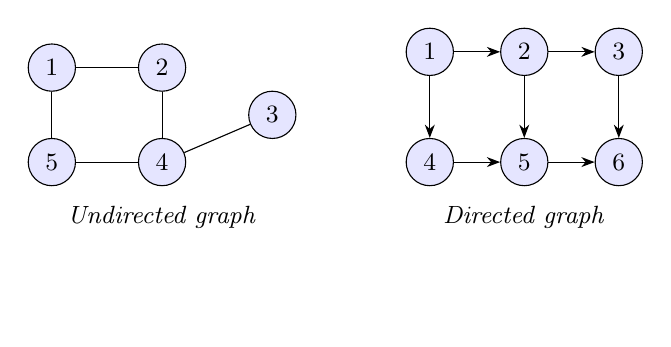
\begin{tikzpicture}[font=\small, every node/.style={circle, draw, fill=blue!10,
                    inner sep=2pt, minimum size=0.6cm}]
  % Undirected graph
  \node (1u) at (0, 1.2) {1};
  \node (2u) at (1.4, 1.2) {2};
  \node (3u) at (2.8, 0.6) {3};
  \node (4u) at (1.4, 0) {4};
  \node (5u) at (0, 0) {5};
  \draw (1u)--(2u); \draw (1u)--(5u); \draw (2u)--(4u);
  \draw (3u)--(4u); \draw (4u)--(5u);
  \node[draw=none, fill=none] at (1.4, -0.7) {\textit{Undirected graph}};

  % Directed graph
  \begin{scope}[xshift=4.8cm, ->, >=Stealth]
  \node (1d) at (0, 1.4) {1};
  \node (2d) at (1.2, 1.4) {2};
  \node (3d) at (2.4, 1.4) {3};
  \node (4d) at (0, 0) {4};
  \node (5d) at (1.2, 0) {5};
  \node (6d) at (2.4, 0) {6};
  \draw (1d)--(2d); \draw (2d)--(3d);
  \draw (4d)--(5d); \draw (5d)--(6d);
  \draw (1d)--(4d); \draw (2d)--(5d); \draw (3d)--(6d);
  \node[draw=none, fill=none] at (1.2, -0.7) {\textit{Directed graph}};
  \end{scope}
\end{tikzpicture}
\end{center}

\subsubsection{Adjacency Lists}

We maintain an array $\mathit{Adj}$ of $|V|$ lists: the list for $u$ contains
all vertices $v$ such that $(u, v) \in E$. We denote this as $G.\mathit{Adj}[u]$ in
algorithms.

\begin{center}
\renewcommand{\arraystretch}{1.25}
\begin{tabular}{lll}
\toprule
\textbf{Operation} & \textbf{Cost} & \\
\midrule
Space & $\Theta(V + E)$ & compact for sparse graphs \\
List neighbors of $u$ & $\Theta(\deg(u))$ & \\
Test $(u,v) \in E$ & $O(\deg(u))$ & \\
\bottomrule
\end{tabular}
\end{center}

\subsubsection{Adjacency Matrix}

A $|V| \times |V|$ matrix where $a_{ij} = 1$ if $(i,j) \in E$, and 0 otherwise.

\begin{center}
\renewcommand{\arraystretch}{1.25}
\begin{tabular}{lll}
\toprule
\textbf{Operation} & \textbf{Cost} & \\
\midrule
Space & $\Theta(V^2)$ & dense, simple to implement \\
List neighbors of $u$ & $\Theta(V)$ & \\
Test $(u,v) \in E$ & $\Theta(1)$ & \\
\bottomrule
\end{tabular}
\end{center}

\begin{remark}{Choice of Representation}{graphrep}
Both representations can be extended to weighted graphs.
For \emph{sparse} graphs ($|E| \ll |V|^2$), adjacency lists are
preferable for space. The matrix is advantageous when edge membership
is tested frequently.
\end{remark}

% ─────────────────────────────────────────────────────────────────────────────
\subsection{Breadth-First Search (BFS)}

\begin{definition}{Breadth-First Search (BFS)}{bfs}
\textbf{Input:} graph $G = (V,E)$ (directed or undirected), source vertex $s \in V$.

\textbf{Output:} for every vertex $v$, $v.d$ = shortest distance (in number of
edges) from $s$ to $v$.
\end{definition}

\textbf{Idea:} send out a wave from $s$. It reaches all vertices at distance 1 first,
then at distance 2, etc. We use a \emph{queue} (FIFO).

\subsubsection{Pseudocode}

\begin{algorithm}[H]
\caption{BFS($G$, $s$)}
\begin{algorithmic}[1]
\For{each vertex $u \in G.V \setminus \{s\}$}
    \State $u.d \leftarrow \infty$
\EndFor
\State $s.d \leftarrow 0$
\State $Q \leftarrow \emptyset$;\; \textsc{Enqueue}$(Q, s)$
\While{$Q \ne \emptyset$}
    \State $u \leftarrow \textsc{Dequeue}(Q)$
    \For{each $v \in G.\mathit{Adj}[u]$}
        \If{$v.d = \infty$}           \AlgComment{$v$ not yet discovered}
            \State $v.d \leftarrow u.d + 1$
            \State \textsc{Enqueue}$(Q, v)$
        \EndIf
    \EndFor
\EndWhile
\end{algorithmic}
\end{algorithm}

\subsubsection{BFS Example}

Graph with 9 vertices $\{s, a, b, c, d, e, f, g, h\}$ from source $s$:

\begin{center}
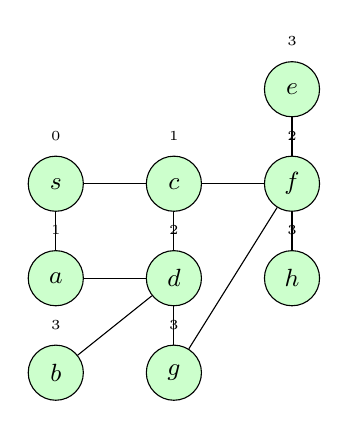
\begin{tikzpicture}[font=\small,
    node/.style={circle, draw, fill=blue!8, minimum size=0.7cm, inner sep=1pt},
    done/.style={circle, draw, fill=green!20, minimum size=0.7cm, inner sep=1pt}]
  % Layout matching the lecture slides
  \node[done] (s) at (0, 1.2) {$s$}; \node[above=2pt] at (s.north) {\tiny 0};
  \node[done] (a) at (0, 0)   {$a$}; \node[above=2pt] at (a.north) {\tiny 1};
  \node[done] (c) at (1.5,1.2){$c$}; \node[above=2pt] at (c.north) {\tiny 1};
  \node[done] (d) at (1.5,0)  {$d$}; \node[above=2pt] at (d.north) {\tiny 2};
  \node[done] (f) at (3.0,1.2){$f$}; \node[above=2pt] at (f.north) {\tiny 2};
  \node[done] (b) at (0,-1.2) {$b$}; \node[above=2pt] at (b.north) {\tiny 3};
  \node[done] (e) at (3.0,2.4){$e$}; \node[above=2pt] at (e.north) {\tiny 3};
  \node[done] (g) at (1.5,-1.2){$g$};\node[above=2pt] at (g.north) {\tiny 3};
  \node[done] (h) at (3.0,0)   {$h$}; \node[above=2pt] at (h.north) {\tiny 3};

  \draw (s)--(a); \draw (s)--(c);
  \draw (a)--(d); \draw (c)--(d); \draw (c)--(f);
  \draw (d)--(b); \draw (d)--(g);
  \draw (f)--(e); \draw (f)--(h); \draw (f)--(g);
\end{tikzpicture}
\end{center}

The discovery order is: $s \to a, c \to d \to f, b \to e, g, h$.
The final distances are indeed the distances in the graph.

\subsubsection{Analysis}

\begin{complexity}{BFS}{bfscplx}
\begin{itemize}[noitemsep]
  \item Each vertex is enqueued at most once: $O(V)$.
  \item Each edge is examined at most once (directed) or twice
        (undirected): $O(E)$.
  \item \textbf{Total complexity: $O(V + E)$.}
\end{itemize}
\end{complexity}

\textbf{Note:} BFS does not necessarily visit all vertices (only those
reachable from $s$). One can record the \emph{BFS tree} by storing
the edge that discovered each vertex ($v.\pi \leftarrow u$).

% ─────────────────────────────────────────────────────────────────────────────
\subsection{Depth-First Search (DFS)}

\begin{definition}{Depth-First Search (DFS)}{dfs}
\textbf{Input:} graph $G = (V,E)$, directed or undirected.

\textbf{Output:} for every vertex $v$, two timestamps:
$v.d$ (\emph{discovery} time) and $v.f$ (\emph{finishing} time).
\end{definition}

\textbf{Idea:} explore each edge as far as possible before backtracking.
As soon as a vertex is discovered, we explore from it (unlike BFS which
explores nearby vertices first). We restart from a new undiscovered
vertex if necessary.

\subsubsection{Vertex Colors}

During execution, each vertex has a color:
\begin{itemize}[noitemsep]
  \item \textbf{WHITE}: undiscovered.
  \item \textbf{GRAY}: discovered but not finished (exploration in progress from it).
  \item \textbf{BLACK}: finished (everything reachable from it has been explored).
\end{itemize}

\subsubsection{Pseudocode}

\begin{algorithm}[H]
\caption{DFS($G$)}
\begin{algorithmic}[1]
\For{each vertex $u \in G.V$}
    \State $u.\mathit{color} \leftarrow \text{WHITE}$
\EndFor
\State $\mathit{time} \leftarrow 0$
\For{each vertex $u \in G.V$}
    \If{$u.\mathit{color} = \text{WHITE}$}
        \State \Call{DFS-Visit}{$G$, $u$}
    \EndIf
\EndFor
\end{algorithmic}
\end{algorithm}

\begin{algorithm}[H]
\caption{DFS-Visit($G$, $u$)}
\begin{algorithmic}[1]
\State $\mathit{time} \leftarrow \mathit{time} + 1$
\State $u.d \leftarrow \mathit{time}$             \AlgComment{discovery timestamp}
\State $u.\mathit{color} \leftarrow \text{GRAY}$
\For{each $v \in G.\mathit{Adj}[u]$}
    \If{$v.\mathit{color} = \text{WHITE}$}
        \State \Call{DFS-Visit}{$G$, $v$}
    \EndIf
\EndFor
\State $u.\mathit{color} \leftarrow \text{BLACK}$
\State $\mathit{time} \leftarrow \mathit{time} + 1$
\State $u.f \leftarrow \mathit{time}$             \AlgComment{finishing timestamp}
\end{algorithmic}
\end{algorithm}

\subsubsection{DFS Example}

Graph with 8 vertices $\{a,b,c,d,e,f,g,h\}$, timestamps $d/f$:

\begin{center}
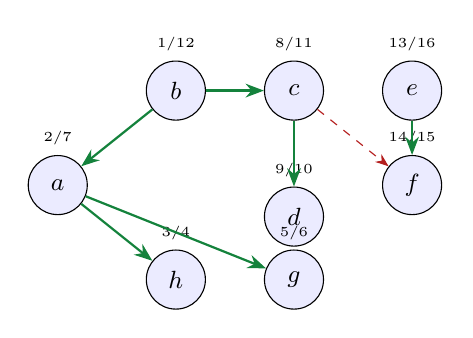
\begin{tikzpicture}[font=\small,
    node/.style={circle, draw, fill=blue!8, minimum size=0.75cm, inner sep=1pt}]
  \node[node] (b) at (1.5, 2.4) {$b$}; \node[above=0pt] at (b.north) {\tiny 1/12};
  \node[node] (c) at (3.0, 2.4) {$c$}; \node[above=0pt] at (c.north) {\tiny 8/11};
  \node[node] (e) at (4.5, 2.4) {$e$}; \node[above=0pt] at (e.north) {\tiny 13/16};
  \node[node] (a) at (0,   1.2) {$a$}; \node[above=0pt] at (a.north) {\tiny 2/7};
  \node[node] (d) at (3.0, 0.8) {$d$}; \node[above=0pt] at (d.north) {\tiny 9/10};
  \node[node] (f) at (4.5, 1.2) {$f$}; \node[above=0pt] at (f.north) {\tiny 14/15};
  \node[node] (h) at (1.5, 0)  {$h$};  \node[above=0pt] at (h.north) {\tiny 3/4};
  \node[node] (g) at (3.0, 0)  {$g$};  \node[above=0pt] at (g.north) {\tiny 5/6};

  % Tree edges
  \draw[->, >=Stealth, keygreen, thick] (b)--(a);
  \draw[->, >=Stealth, keygreen, thick] (a)--(h);
  \draw[->, >=Stealth, keygreen, thick] (a)--(g);
  \draw[->, >=Stealth, keygreen, thick] (b)--(c);
  \draw[->, >=Stealth, keygreen, thick] (c)--(d);
  \draw[->, >=Stealth, keygreen, thick] (e)--(f);
  % Cross/forward edges
  \draw[->, >=Stealth, keyred, dashed] (c)--(f) node[midway, right, font=\tiny]{};
\end{tikzpicture}
\end{center}

The DFS forest here contains two trees rooted at $b$ (time 1) and $e$ (time 13).

\subsubsection{Analysis}

\begin{complexity}{DFS}{dfscplx}
\begin{itemize}[noitemsep]
  \item Each vertex is discovered exactly once: $\Theta(V)$.
  \item Each edge is examined exactly once (directed) or twice
        (undirected): $\Theta(E)$.
  \item \textbf{Total complexity: $\Theta(V + E)$.}
\end{itemize}
\end{complexity}

DFS produces a \textbf{DFS forest}: one or more trees, each originating
from a \textsc{DFS-Visit} call in the main loop.

% ─────────────────────────────────────────────────────────────────────────────
\subsection{Edge Classification (DFS)}

In a DFS, each edge $(u,v)$ can be classified according to its timestamps:

\begin{center}
\renewcommand{\arraystretch}{1.35}
\begin{tabular}{lll}
\toprule
\textbf{Type} & \textbf{Definition} & \textbf{Condition} \\
\midrule
\textbf{Tree edge}    & in the DFS forest & $v$ was WHITE when $(u,v)$ explored \\
\textbf{Back edge}    & $(u,v)$: $u$ is descendant of $v$ & $v.d < u.d < u.f < v.f$ \\
\textbf{Forward edge} & $(u,v)$: $v$ is descendant of $u$, \newline but not via tree & $u.d < v.d < v.f < u.f$ \\
\textbf{Cross edge}   & any other edge & $v.f < u.d$ \\
\bottomrule
\end{tabular}
\end{center}

\begin{remark}{Undirected Graphs}{undirected}
In the DFS of an \emph{undirected} graph, we only obtain tree edges and
back edges — never forward edges or cross edges. Indeed, if $(u,v)$ is examined
from $u$ and $v$ is already GRAY or BLACK, then $v$ is necessarily an ancestor
of $u$ in the current tree, which results in a back edge.
\end{remark}

% ─────────────────────────────────────────────────────────────────────────────
\subsection{Summary: BFS and DFS}

\begin{center}
\renewcommand{\arraystretch}{1.45}
\begin{tabular}{lll}
\toprule
& \textbf{BFS} & \textbf{DFS} \\
\midrule
Structure used & Queue (FIFO) & Stack (recursion) \\
Exploration order & By increasing distance & Depth-first \\
Main output & Distances $v.d$ from $s$ & Timestamps $v.d$, $v.f$ \\
Complexity & $O(V+E)$ & $\Theta(V+E)$ \\
Reaches whole graph & No (from $s$ only) & Yes (if looping through all vertices) \\
Applications & Shortest path (unweighted) & Topological sort, connected components \\
\bottomrule
\end{tabular}
\end{center}

\section{Lecture 13 : Graphs – DFS theorem and topological sort}
% ══════════════════════════════════════════════════════════════════════════════
% Lecture 13: Graphs – DFS Theorems and Topological Sort
% ══════════════════════════════════════════════════════════════════════════════

% ─────────────────────────────────────────────────────────────────────────────
\subsection{Parenthesis Theorem}

DFS timestamps have a strict nested structure:

\begin{theorem}{Parenthesis Theorem}{parenthesis}
For any two vertices $u$ and $v$, exactly one of the following three situations occurs:
\begin{enumerate}
  \item The intervals $[u.d,\, u.f]$ and $[v.d,\, v.f]$ are \textbf{disjoint}, and
        neither $u$ nor $v$ is an ancestor of the other.
  \item $[v.d,\, v.f] \subset [u.d,\, u.f]$ (i.e., $u.d < v.d < v.f < u.f$)
        and $v$ is a \textbf{descendant} of $u$.
  \item $[u.d,\, u.f] \subset [v.d,\, v.f]$ (i.e., $v.d < u.d < u.f < v.f$)
        and $u$ is a \textbf{descendant} of $v$.
\end{enumerate}
\end{theorem}

\textbf{Illustration.} Using the example from Lecture 12 ($b$: 1/12, $a$: 2/7, $h$: 3/4,
$g$: 5/6, $c$: 8/11, $d$: 9/10, $e$: 13/16, $f$: 14/15):

\begin{center}
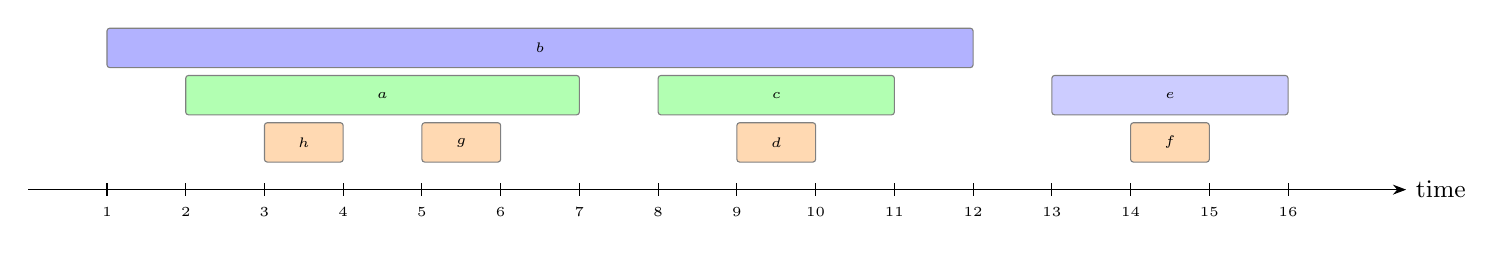
\begin{tikzpicture}[font=\small, >=Stealth]
  % Timeline
  \draw[->] (0,0) -- (17.5,0) node[right] {time};
  \foreach \t in {1,...,16}{
    \draw (\t, 0.08) -- (\t, -0.08);
    \node[below, font=\tiny] at (\t, -0.1) {\t};
  }
  % Intervals
  \foreach \label/\s/\e/\y/\col in {
    $b$/1/12/1.8/blue!30,
    $a$/2/7/1.2/green!30,
    $h$/3/4/0.6/orange!30,
    $g$/5/6/0.6/orange!30,
    $c$/8/11/1.2/green!30,
    $d$/9/10/0.6/orange!30,
    $e$/13/16/1.2/blue!20,
    $f$/14/15/0.6/orange!30}{
    \draw[fill=\col, draw=gray, rounded corners=1pt]
          (\s, \y-0.25) rectangle (\e, \y+0.25);
    \node[font=\tiny\bfseries] at ({(\s+\e)/2}, \y) {\label};
  }
\end{tikzpicture}
\end{center}

We see that the intervals are either nested (ancestor/descendant) or disjoint
(no descendant relationship). They never partially overlap.

% ─────────────────────────────────────────────────────────────────────────────
\subsection{White-Path Theorem}

\begin{theorem}{White-Path Theorem}{whitepath}
In a DFS forest of a graph $G$, vertex $v$ is a \textbf{descendant} of $u$
if and only if at time $u.d$ (when $u$ is just discovered), there exists a
path from $u$ to $v$ consisting \textbf{entirely of WHITE vertices}
(not yet discovered), with the exception of $u$ itself which has just been colored GRAY.
\end{theorem}

This theorem fully characterizes the descendant relationship in the DFS forest:
$v$ will be in $u$'s subtree precisely if such a white path exists
at the moment $u$ is discovered.

% ══════════════════════════════════════════════════════════════════════════════
\section*{Topological Sort}
\addcontentsline{toc}{subsection}{Topological Sort}
% ══════════════════════════════════════════════════════════════════════════════

% ─────────────────────────────────────────────────────────────────────────────
\subsection{Definition}

\begin{definition}{Topological Sort}{topo}
\textbf{Input:} a directed acyclic graph (DAG) $G = (V, E)$.

\textbf{Output:} a linear ordering of vertices such that for every edge
$(u, v) \in E$, $u$ appears before $v$ in the ordering.
\end{definition}

\textbf{Motivating example:} the order in which one gets dressed in the morning.
If you must put on socks before shoes, and underwear
before pants, a topological sort provides an order consistent with all these
constraints.

\begin{remark}{DAG and Applicability}{dagrem}
A topological sort exists only if the graph is \textbf{acyclic} (DAG).
In the presence of a cycle, no linear ordering can satisfy all
precedence constraints.
\end{remark}

% ─────────────────────────────────────────────────────────────────────────────
\subsection{Characterizing DAGs via DFS}

\begin{theorem}{DAG $\Leftrightarrow$ No DFS Back Edge}{daglem}
A directed graph $G$ is acyclic if and only if a DFS of $G$ produces
\textbf{no back edges}.
\end{theorem}

\begin{proof}
\textbf{Back edge $\Rightarrow$ cycle.}
Suppose a back edge $(u, v)$ exists. Then $v$ is an ancestor of $u$
in the DFS forest, so there is a path from $v$ to $u$ in $G$. The back edge
$(u, v)$ closes this path into a cycle.

\begin{center}
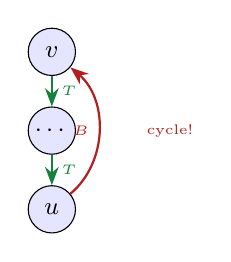
\begin{tikzpicture}[font=\small, >=Stealth,
    node/.style={circle, draw, fill=blue!10, minimum size=0.6cm, inner sep=1pt}]
  \node[node] (v) at (1, 2) {$v$};
  \node[node] (m) at (1, 1) {$\cdots$};
  \node[node] (u) at (1, 0) {$u$};
  \draw[->, keygreen, thick] (v) -- (m) node[midway, right, font=\tiny]{$T$};
  \draw[->, keygreen, thick] (m) -- (u) node[midway, right, font=\tiny]{$T$};
  \draw[->, keyred, thick, bend right=50] (u) to node[left, font=\tiny]{$B$} (v);
  \node[keyred, font=\tiny] at (2.5, 1) {cycle!};
\end{tikzpicture}
\end{center}

\textbf{Cycle $\Rightarrow$ back edge.}
Let $C$ be a cycle in $G$ and $v$ be the first vertex of $C$ discovered by DFS.
Let $(u, v)$ be the edge preceding $v$ in the cycle. At time $v.d$, the vertices
of $C$ form a white path from $v$ to $u$. By the white-path theorem,
$u$ becomes a descendant of $v$, so the edge $(u, v)$ is a back edge.
\end{proof}

% ─────────────────────────────────────────────────────────────────────────────
\subsection{Algorithm}

\begin{algorithm}[H]
\caption{Topological-Sort($G$)}
\begin{algorithmic}[1]
\State Call \textsc{DFS}($G$) to compute finishing times $v.f$ for all $v$
\State \Return the vertices in \textbf{decreasing} order of finishing times $v.f$
\end{algorithmic}
\end{algorithm}

\textbf{Efficient implementation:} explicit sorting is not necessary.
One can insert each vertex at the \emph{head} of a linked list at the moment
it is finished (colored BLACK). At the end of the DFS, the list contains the vertices
in topological order.

\begin{complexity}{Topological-Sort}{topocplx}
\textbf{Complexity: $\Theta(V + E)$} — identical to DFS complexity.
\end{complexity}

% ─────────────────────────────────────────────────────────────────────────────
\subsection{Proof of Correctness}

We must show that if $(u, v) \in E$, then $v.f < u.f$ (so $u$ appears before
$v$ in the decreasing order of finishing times).

When edge $(u,v)$ is explored during DFS, $u$ is GRAY. Three cases for $v$:

\begin{center}
\renewcommand{\arraystretch}{1.4}
\begin{tabular}{cll}
\toprule
\textbf{Color of $v$} & \textbf{Consequence} & \textbf{Result} \\
\midrule
GRAY & $v$ would be an ancestor of $u$ & Back edge $\Rightarrow$ cycle $\Rightarrow$ contradiction \\
WHITE & $v$ becomes descendant of $u$ & By parenthesis: $u.d < v.d < v.f < u.f$ \\
BLACK & $v$ already finished, $u$ not yet & Directly $v.f < u.f$ \\
\bottomrule
\end{tabular}
\end{center}

In all non-contradictory cases, we indeed obtain $v.f < u.f$. \qed

% ─────────────────────────────────────────────────────────────────────────────
\subsection{Example}

\begin{center}
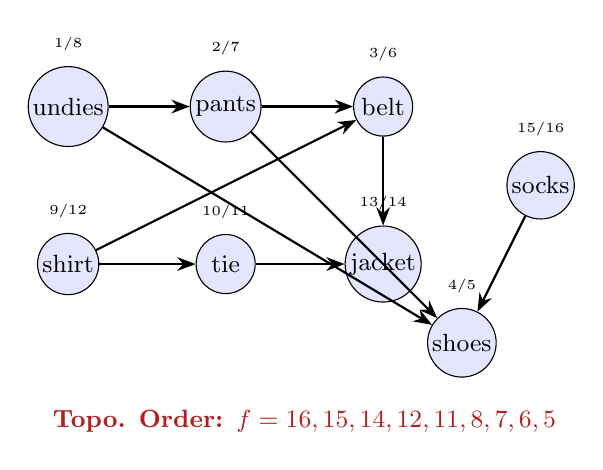
\begin{tikzpicture}[font=\small, >=Stealth,
    node/.style={circle, draw, fill=blue!10, minimum size=0.75cm, inner sep=1pt}]
  % Nodes with DFS timestamps
  \node[node] (undies) at (0, 2)    {\small undies}; \node[above=2pt] at (undies.north) {\tiny 1/8};
  \node[node] (pants)  at (2, 2)    {\small pants}; \node[above=2pt] at (pants.north)  {\tiny 2/7};
  \node[node] (belt)   at (4, 2)    {\small belt}; \node[above=2pt] at (belt.north)   {\tiny 3/6};
  \node[node] (shirt)  at (0, 0)    {\small shirt}; \node[above=2pt] at (shirt.north)  {\tiny 9/12};
  \node[node] (tie)    at (2, 0)    {\small tie};  \node[above=2pt] at (tie.north)    {\tiny 10/11};
  \node[node] (jacket) at (4, 0)    {\small jacket}; \node[above=2pt] at (jacket.north) {\tiny 13/14};
  \node[node] (socks)  at (6, 1)    {\small socks}; \node[above=2pt] at (socks.north) {\tiny 15/16};
  \node[node] (shoes)  at (5, -1)   {\small shoes}; \node[above=2pt] at (shoes.north)  {\tiny 4/5};
  \draw[->,thick] (undies)--(pants);
  \draw[->,thick] (undies)--(shoes);
  \draw[->,thick] (pants)--(belt);
  \draw[->,thick] (pants)--(shoes);
  \draw[->,thick] (belt)--(jacket);
  \draw[->,thick] (shirt)--(belt);
  \draw[->,thick] (shirt)--(tie);
  \draw[->,thick] (tie)--(jacket);
  \draw[->,thick] (socks)--(shoes);
  % Topological order arrow
  \node[draw=none, fill=none, keyred, font=\bfseries\small] at (3, -2)
        {Topo. Order: $f=16,15,14,12,11,8,7,6,5$};
\end{tikzpicture}
\end{center}

The topological sort (decreasing finishing times) yields a valid
dressing order: each garment appears after those that must be put on before it.

% ─────────────────────────────────────────────────────────────────────────────
\subsection{Lecture Summary}

\begin{tcolorbox}[colback=lightblue, colframe=keyblue, fonttitle=\bfseries,
                  title={Key Points}]
\begin{itemize}[noitemsep]
  \item \textbf{Parenthesis Theorem:} the intervals $[u.d, u.f]$ are either
        nested or disjoint — never partially overlapping.
  \item \textbf{White-Path Theorem:} $v$ is a descendant of $u$ iff there exists
        a white path from $u$ to $v$ at time $u.d$.
  \item \textbf{DAG $\Leftrightarrow$ No back edge:} a tool for detecting
        cycles.
  \item \textbf{Topological Sort:} DFS + decreasing order of finishing times.
        Complexity $\Theta(V+E)$.
\end{itemize}
\end{tcolorbox}

\section{Lecture 14 : Composantes Fortement Connexes et Réseaux de Flot}
% ══════════════════════════════════════════════════════════════════════════════
% Lecture 14: Strongly Connected Components and Flow Networks
% ══════════════════════════════════════════════════════════════════════════════

% ══════════════════════════════════════════════════════════════════════════════
\section*{Strongly Connected Components (SCC)}
\addcontentsline{toc}{subsection}{Strongly Connected Components}
% ══════════════════════════════════════════════════════════════════════════════

% ─────────────────────────────────────────────────────────────────────────────
\subsection{Definition}

\begin{definition}{Strongly Connected Component}{scc}
A \textbf{strongly connected component (SCC)} of a directed graph
$G = (V, E)$ is a \emph{maximal} set of vertices $C \subseteq V$
such that for every $u, v \in C$, there is a path from $u$ to $v$
\emph{and} a path from $v$ to $u$ (denoted $u \leadsto v$ and $v \leadsto u$).
\end{definition}

\textbf{Example:} on a graph with 10 vertices $\{a, b, c, d, e, f, g, h, i, j\}$,
the SCCs may group as $\{a, b, e, f\}$, $\{c, d, h\}$, $\{g\}$, $\{i, j\}$
depending on the edges present. A subset that is not maximal, or in which
two vertices are not mutually reachable, is not an SCC.

% ─────────────────────────────────────────────────────────────────────────────
\subsection{Component Graph}

\begin{definition}{Component Graph $G^{SCC}$}{gscc}
For a directed graph $G = (V, E)$, the component graph
$G^{SCC} = (V^{SCC}, E^{SCC})$ is defined by:
\begin{itemize}[noitemsep]
  \item $V^{SCC}$ contains one vertex for each SCC of $G$.
  \item $E^{SCC}$ contains an edge between two SCCs if there exists an edge
        between the corresponding SCCs in $G$.
\end{itemize}
\end{definition}

\begin{theorem}{$G^{SCC}$ is a DAG}{sccdag}
The component graph $G^{SCC}$ is always a directed acyclic graph.
\end{theorem}

This follows from the fact that if a cycle existed in $G^{SCC}$, all involved SCCs
would form a single SCC, which contradicts their definition.

% ─────────────────────────────────────────────────────────────────────────────
\subsection{Kosaraju's Algorithm}

\begin{algorithm}[H]
\caption{SCC($G$)}
\begin{algorithmic}[1]
\State Call \textsc{DFS}($G$) to compute finishing times $u.f$ for all $u$
\State Compute the transpose graph $G^T$   \AlgComment{reverse all edges}
\State Call \textsc{DFS}($G^T$) processing vertices in
       \textbf{decreasing} order of $u.f$ calculated in step 1
\State \Return each tree of the DFS forest from step 3 as a distinct SCC
\end{algorithmic}
\end{algorithm}

\textbf{Transpose Graph $G^T$:}
$G^T = (V, E^T)$ where $E^T = \{(u,v) : (v,u) \in E\}$ — all edges are
reversed. $G^T$ is calculated in $\Theta(V + E)$ using adjacency lists, and
$G$ and $G^T$ possess exactly the same SCCs.

\begin{complexity}{Kosaraju's SCC}{scccplx}
Each step executes in $\Theta(V + E)$, so the
\textbf{total complexity is $\Theta(V + E)$}.
\end{complexity}

\subsubsection{Intuition of Correctness}

The first DFS orders the SCCs in topological order in $G^{SCC}$ (which is a DAG).
The second DFS on $G^T$ starts from the SCC with the largest $u.f$, and in $G^T$ the
edges between SCCs are reversed: one cannot therefore "escape" to another
SCC. Each tree of the second DFS is exactly one SCC.

\subsubsection{Example}

On a graph with 10 vertices, the first DFS (on $G$) produces the
following timestamps (reading the slides: $d$: 1/12, $i$: 10/11, $h$: 2/5, $c$: 3/4,
$j$: 7/8, $e$: 6/9, $a$: 14/19, $b$: 15/16, $f$: 17/18, $g$: 13/20).

The second DFS on $G^T$ starts from $g$ ($f=20$), then $a$ ($f=19$), etc., and
each tree formed corresponds to an SCC:

\begin{center}
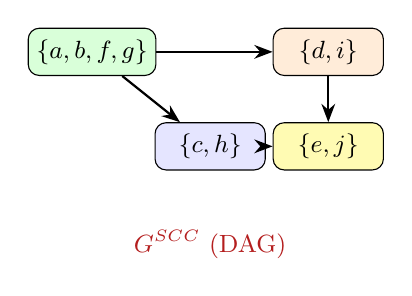
\begin{tikzpicture}[font=\small, >=Stealth,
    scc/.style={draw, rounded corners, fill=blue!10,
                minimum width=1.4cm, minimum height=0.6cm, inner sep=3pt}]
  \node[scc, fill=green!15]  (s1) at (0, 0)   {$\{a,b,f,g\}$};
  \node[scc, fill=orange!15] (s2) at (3, 0)   {$\{d,i\}$};
  \node[scc, fill=blue!10]   (s3) at (1.5,-1.2){$\{c,h\}$};
  \node[scc, fill=yellow!30] (s4) at (3,-1.2)  {$\{e,j\}$};
  \draw[->, thick] (s1) -- (s2);
  \draw[->, thick] (s1) -- (s3);
  \draw[->, thick] (s2) -- (s4);
  \draw[->, thick] (s3) -- (s4);
  \node[below=4pt, keyred, font=\small] at (1.5, -2) {$G^{SCC}$ (DAG)};
\end{tikzpicture}
\end{center}

% ══════════════════════════════════════════════════════════════════════════════
\section*{Flow Networks}
\addcontentsline{toc}{subsection}{Flow Networks}
% ══════════════════════════════════════════════════════════════════════════════

% ─────────────────────────────────────────────────────────────────────────────
\subsection{Definition}

\begin{definition}{Flow network}{flownet}
A \textbf{flow network} is a directed graph $G = (V, E)$ where:
\begin{itemize}[noitemsep]
  \item Each edge $(u,v)$ has a \textbf{capacity} $c(u,v) \ge 0$
        (and $c(u,v) = 0$ if $(u,v) \notin E$).
  \item There is a \textbf{source} $s$ and a \textbf{sink} $t$.
  \item We assume the absence of anti-parallel edges (without loss of generality).
\end{itemize}
\end{definition}

\textbf{Example:} transporting Gruyère cheese ($s$) to Lausanne ($t$) via
intermediate cities, each route having a maximum capacity.

\begin{center}
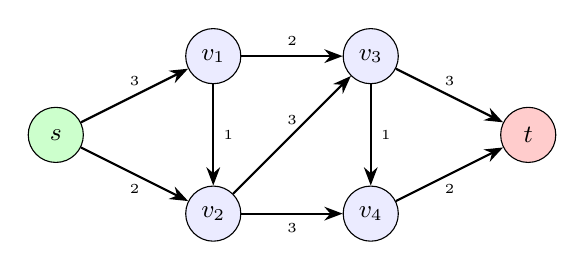
\begin{tikzpicture}[font=\small, >=Stealth,
    node/.style={circle, draw, fill=blue!8, minimum size=0.7cm, inner sep=1pt}]
  \node[node, fill=green!20] (s)  at (0, 1)   {$s$};
  \node[node]                (v1) at (2, 2)   {$v_1$};
  \node[node]                (v2) at (2, 0)   {$v_2$};
  \node[node]                (v3) at (4, 2)   {$v_3$};
  \node[node]                (v4) at (4, 0)   {$v_4$};
  \node[node, fill=red!20]   (t)  at (6, 1)   {$t$};
  \draw[->, thick] (s)  -- node[above, font=\tiny]{3} (v1);
  \draw[->, thick] (s)  -- node[below, font=\tiny]{2} (v2);
  \draw[->, thick] (v1) -- node[above, font=\tiny]{2} (v3);
  \draw[->, thick] (v1) -- node[right, font=\tiny]{1} (v2);
  \draw[->, thick] (v2) -- node[below, font=\tiny]{3} (v4);
  \draw[->, thick] (v2) -- node[above, font=\tiny]{3} (v3);
  \draw[->, thick] (v3) -- node[above, font=\tiny]{3} (t);
  \draw[->, thick] (v4) -- node[below, font=\tiny]{2} (t);
  \draw[->, thick] (v3) -- node[right, font=\tiny]{1} (v4);
\end{tikzpicture}
\end{center}

\subsubsection{Removing anti-parallel edges}

If the graph contains $(u,v)$ and $(v,u)$, we replace $(u,v)$ with two edges
$(u, v')$ and $(v', v)$ with $c(u,v') = c(v',v) = c(u,v)$, by introducing a
dummy vertex $v'$. Repeat for each anti-parallel pair ($O(E)$ times).

% ─────────────────────────────────────────────────────────────────────────────
\subsection{Definition of a Flow}

\begin{definition}{Flow}{flow}
A \textbf{flow} is a function $f : V \times V \to \mathbb{R}$ satisfying:

\textbf{Capacity constraint:} $\forall\, u, v \in V$,
\[
  0 \le f(u,v) \le c(u,v).
\]

\textbf{Flow conservation:} $\forall\, u \in V \setminus \{s, t\}$,
\[
  \underbrace{\sum_{v \in V} f(v,u)}_{\text{incoming flow}} =
  \underbrace{\sum_{v \in V} f(u,v)}_{\text{outgoing flow}}.
\]
\end{definition}

The \textbf{value} of flow $f$ is:
\[
  |f| = \sum_{v \in V} f(s,v) - \sum_{v \in V} f(v,s)
       = \text{total flow exiting the source}.
\]

\textbf{Example} (network above, flow with value $|f| = 4$):

\begin{center}
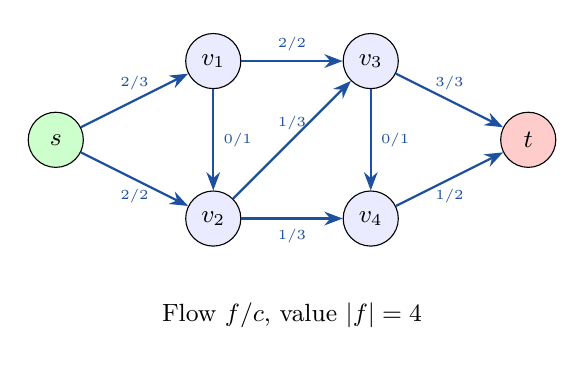
\begin{tikzpicture}[font=\small, >=Stealth,
    node/.style={circle, draw, fill=blue!8, minimum size=0.7cm, inner sep=1pt}]
  \node[node, fill=green!20] (s)  at (0, 1)   {$s$};
  \node[node]                (v1) at (2, 2)   {$v_1$};
  \node[node]                (v2) at (2, 0)   {$v_2$};
  \node[node]                (v3) at (4, 2)   {$v_3$};
  \node[node]                (v4) at (4, 0)   {$v_4$};
  \node[node, fill=red!20]   (t)  at (6, 1)   {$t$};
  \draw[->, thick, keyblue] (s)  -- node[above, font=\tiny]{2/3} (v1);
  \draw[->, thick, keyblue] (s)  -- node[below, font=\tiny]{2/2} (v2);
  \draw[->, thick, keyblue] (v1) -- node[above, font=\tiny]{2/2} (v3);
  \draw[->, thick, keyblue] (v1) -- node[right, font=\tiny]{0/1} (v2);
  \draw[->, thick, keyblue] (v2) -- node[below, font=\tiny]{1/3} (v4);
  \draw[->, thick, keyblue] (v2) -- node[above, font=\tiny]{1/3} (v3);
  \draw[->, thick, keyblue] (v3) -- node[above, font=\tiny]{3/3} (t);
  \draw[->, thick, keyblue] (v4) -- node[below, font=\tiny]{1/2} (t);
  \draw[->, thick, keyblue] (v3) -- node[right, font=\tiny]{0/1} (v4);
  \node[below=4pt, font=\small] at (3, -0.8) {Flow $f/c$, value $|f|=4$};
\end{tikzpicture}
\end{center}

% ─────────────────────────────────────────────────────────────────────────────
\subsection{Residual Network}

\begin{definition}{Residual Network $G_f$}{residual}
Given a flow $f$ in $G = (V, E)$, the \textbf{residual capacity} is:
\[
  c_f(u,v) =
  \begin{cases}
    c(u,v) - f(u,v) & \text{if } (u,v) \in E \quad (\text{remaining capacity})\\
    f(v,u)          & \text{if } (v,u) \in E \quad (\text{cancellable flow}) \\
    0               & \text{otherwise.}
  \end{cases}
\]
The \textbf{residual network} is $G_f = (V, E_f)$ where
$E_f = \{(u,v) \in V \times V : c_f(u,v) > 0\}$.
\end{definition}

\begin{remark}{Role of reversed residual edges}{residualinv}
The reversed edges $(v,u)$ in $G_f$ represent the possibility of
\emph{reducing} the flow on $(u,v)$, which is equivalent to rerouting it elsewhere.
It is this mechanism that allows the algorithm to correct bad initial choices.
\end{remark}

% ─────────────────────────────────────────────────────────────────────────────
\subsection{Ford-Fulkerson Method}

\begin{algorithm}[H]
\caption{Ford-Fulkerson-Method($G$, $s$, $t$)}
\begin{algorithmic}[1]
\State Initialize $f(u,v) \leftarrow 0$ for all $(u,v)$
\While{there exists an \textbf{augmenting path} $p$ from $s$ to $t$ in $G_f$}
    \State \textbf{Augment} the flow $f$ along $p$
\EndWhile
\State \Return $f$
\end{algorithmic}
\end{algorithm}

An \textbf{augmenting path} is a simple path from $s$ to $t$ in the residual
network $G_f$. We send a flow equal to the \textbf{minimum residual capacity}
on this path:
\[
  c_f(p) = \min_{(u,v) \in p} c_f(u,v).
\]

For each edge $(u,v) \in p$, the flow is updated by:
$f(u,v) \leftarrow f(u,v) + c_f(p) - c_f(v,u)$ (taking into account reversed 
edges).

\subsubsection{Step-by-step example}

Diamond graph with a central edge of capacity 1 (the two paths of capacity 1
each):

\begin{center}
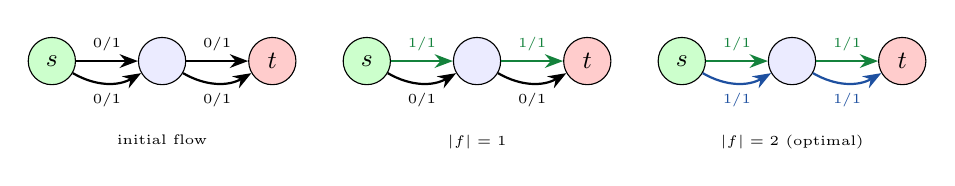
\begin{tikzpicture}[font=\small, >=Stealth,
    node/.style={circle, draw, fill=blue!8, minimum size=0.6cm, inner sep=1pt}]
  % Step 1: initial flow 0
  \begin{scope}[xshift=0cm]
    \node[node, fill=green!20] (s1) at (0,1)  {$s$};
    \node[node]                (m1) at (1.4,1){};
    \node[node, fill=red!20]   (t1) at (2.8,1){$t$};
    \draw[->,thick] (s1) -- node[above,font=\tiny]{0/1} (m1);
    \draw[->,thick] (m1) -- node[above,font=\tiny]{0/1} (t1);
    \draw[->,thick] (s1) to[bend right=30] node[below,font=\tiny]{0/1} (m1);
    \draw[->,thick] (m1) to[bend right=30] node[below,font=\tiny]{0/1} (t1);
    \node[below=6pt,font=\tiny] at (1.4,0.4) {initial flow};
  \end{scope}
  % Step 2: after 1st augmenting path
  \begin{scope}[xshift=4cm]
    \node[node, fill=green!20] (s2) at (0,1)  {$s$};
    \node[node]                (m2) at (1.4,1){};
    \node[node, fill=red!20]   (t2) at (2.8,1){$t$};
    \draw[->,thick,keygreen] (s2) -- node[above,font=\tiny]{1/1} (m2);
    \draw[->,thick,keygreen] (m2) -- node[above,font=\tiny]{1/1} (t2);
    \draw[->,thick] (s2) to[bend right=30] node[below,font=\tiny]{0/1} (m2);
    \draw[->,thick] (m2) to[bend right=30] node[below,font=\tiny]{0/1} (t2);
    \node[below=6pt,font=\tiny] at (1.4,0.4) {$|f|=1$};
  \end{scope}
  % Step 3: lower path, flow=2
  \begin{scope}[xshift=8cm]
    \node[node, fill=green!20] (s3) at (0,1)  {$s$};
    \node[node]                (m3) at (1.4,1){};
    \node[node, fill=red!20]   (t3) at (2.8,1){$t$};
    \draw[->,thick,keygreen] (s3) -- node[above,font=\tiny]{1/1} (m3);
    \draw[->,thick,keygreen] (m3) -- node[above,font=\tiny]{1/1} (t3);
    \draw[->,thick,keyblue] (s3) to[bend right=30] node[below,font=\tiny]{1/1} (m3);
    \draw[->,thick,keyblue] (m3) to[bend right=30] node[below,font=\tiny]{1/1} (t3);
    \node[below=6pt,font=\tiny] at (1.4,0.4) {$|f|=2$ (optimal)};
  \end{scope}
\end{tikzpicture}
\end{center}

\textbf{Case where reversed edges are necessary.} Without them, a bad
first choice (path passing through the central edge) would stall at $|f|=1$ instead
of 2. The residual network allows "undoing" this choice via a back edge.

% ─────────────────────────────────────────────────────────────────────────────
\subsection{Lecture Summary}

\begin{tcolorbox}[colback=lightblue, colframe=keyblue, fonttitle=\bfseries,
                  title={Key Points}]
\begin{itemize}[noitemsep]
  \item \textbf{SCC:} maximal set of mutually reachable vertices.
  \item \textbf{$G^{SCC}$ is a DAG.}
  \item \textbf{Kosaraju:} 2 DFS ($G$ then $G^T$ in decreasing order of $u.f$).
        Complexity $\Theta(V+E)$.
  \item \textbf{Flow Network:} capacity constraint $0 \le f(u,v) \le c(u,v)$
        and flow conservation at every vertex $\ne s, t$.
  \item \textbf{Residual Network $G_f$:} encodes what can still be sent
        (or cancelled) on each edge.
  \item \textbf{Ford-Fulkerson:} augment along $s \leadsto t$ paths in
        $G_f$ until exhaustion.
\end{itemize}
\end{tcolorbox}

\section{Lecture 15 : Flows and cut - Max-Flow Min-Cut}
% ══════════════════════════════════════════════════════════════════════════════
% Lecture 15: Flows and Cuts – Max-Flow Min-Cut Theorem
% ══════════════════════════════════════════════════════════════════════════════

% ─────────────────────────────────────────────────────────────────────────────
\subsection{Full Example of Ford-Fulkerson}

To illustrate the method, here is the evolution of the flow on a network with 
integer capacities until the optimum $|f| = 29$:

\begin{center}
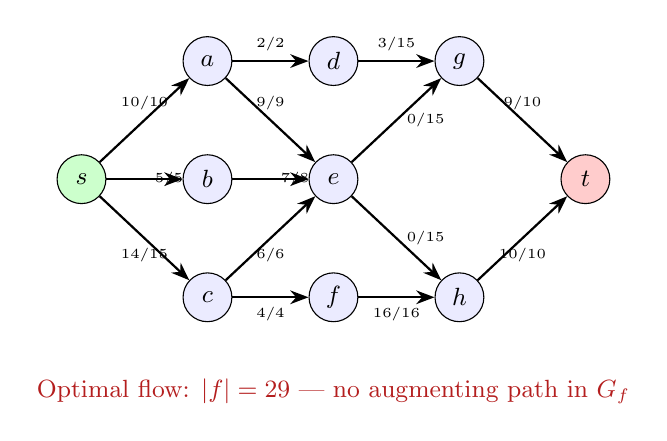
\begin{tikzpicture}[font=\small, >=Stealth,
    node/.style={circle, draw, fill=blue!8, minimum size=0.62cm, inner sep=1pt}]
  \node[node, fill=green!20] (s)  at (0,   1.5) {$s$};
  \node[node]                (a)  at (1.6,  3)  {$a$};
  \node[node]                (b)  at (1.6,  1.5){$b$};
  \node[node]                (c)  at (1.6,  0)  {$c$};
  \node[node]                (d)  at (3.2,  3)  {$d$};
  \node[node]                (e)  at (3.2,  1.5){$e$};
  \node[node]                (f)  at (3.2,  0)  {$f$};
  \node[node]                (g)  at (4.8,  3)  {$g$};
  \node[node]                (h)  at (4.8,  0)  {$h$};
  \node[node, fill=red!20]   (t)  at (6.4,  1.5){$t$};

  % Final optimal flow f/c
  \draw[->,thick] (s) -- node[above,font=\tiny]{10/10}(a);
  \draw[->,thick] (s) -- node[right,font=\tiny]{5/5} (b);
  \draw[->,thick] (s) -- node[below,font=\tiny]{14/15}(c);
  \draw[->,thick] (a) -- node[above,font=\tiny]{2/2} (d);
  \draw[->,thick] (a) -- node[above,font=\tiny]{9/9} (e);
  \draw[->,thick] (b) -- node[right,font=\tiny]{7/8} (e);
  \draw[->,thick] (c) -- node[below,font=\tiny]{4/4} (f);
  \draw[->,thick] (c) -- node[below,font=\tiny]{6/6} (e);
  \draw[->,thick] (d) -- node[above,font=\tiny]{3/15}(g);
  \draw[->,thick] (e) -- node[right,font=\tiny]{0/15}(g);
  \draw[->,thick] (e) -- node[right,font=\tiny]{0/15}(h);
  \draw[->,thick] (f) -- node[below,font=\tiny]{16/16}(h);
  \draw[->,thick] (g) -- node[above,font=\tiny]{9/10} (t);
  \draw[->,thick] (h) -- node[below,font=\tiny]{10/10}(t);
  \node[below=6pt, keyred, font=\small] at (3.2, -0.7)
        {Optimal flow: $|f| = 29$ — no augmenting path in $G_f$};
\end{tikzpicture}
\end{center}

% ══════════════════════════════════════════════════════════════════════════════
\section*{Cuts in Flow Networks}
\addcontentsline{toc}{subsection}{Cuts and Max-Flow Min-Cut Theorem}
% ══════════════════════════════════════════════════════════════════════════════

% ─────────────────────────────────────────────────────────────────────────────
\subsection{Definition of a Cut}

\begin{definition}{Cut}{cut}
A \textbf{cut} of the flow network $G = (V, E)$ is a partition of $V$ into
two sets $S$ and $T = V \setminus S$ such that $s \in S$ and $t \in T$.
\end{definition}

\begin{center}
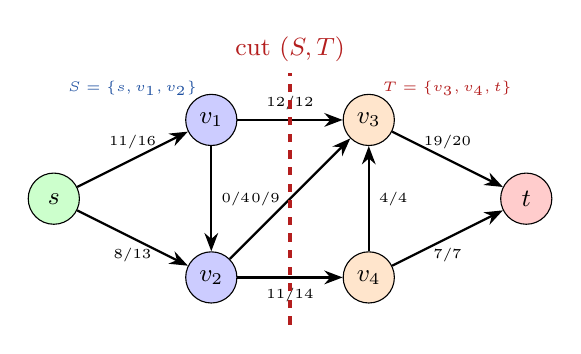
\begin{tikzpicture}[font=\small, >=Stealth,
    node/.style={circle, draw, fill=blue!8, minimum size=0.65cm, inner sep=1pt}]
  \node[node, fill=green!20] (s)  at (0, 1)   {$s$};
  \node[node, fill=blue!20]  (v1) at (2, 2)   {$v_1$};
  \node[node, fill=blue!20]  (v2) at (2, 0)   {$v_2$};
  \node[node, fill=orange!20](v3) at (4, 2)   {$v_3$};
  \node[node, fill=orange!20](v4) at (4, 0)   {$v_4$};
  \node[node, fill=red!20]   (t)  at (6, 1)   {$t$};

  \draw[->, thick] (s)  -- node[above,font=\tiny]{11/16}(v1);
  \draw[->, thick] (s)  -- node[below,font=\tiny]{8/13} (v2);
  \draw[->, thick] (v1) -- node[above,font=\tiny]{12/12}(v3);
  \draw[->, thick] (v1) -- node[right,font=\tiny]{0/4}  (v2);
  \draw[->, thick] (v2) -- node[below,font=\tiny]{11/14}(v4);
  \draw[->, thick] (v2) -- node[left, font=\tiny]{0/9}  (v3);
  \draw[->, thick] (v3) -- node[above,font=\tiny]{19/20}(t);
  \draw[->, thick] (v4) -- node[below,font=\tiny]{7/7}  (t);
  \draw[->, thick] (v4) -- node[right,font=\tiny]{4/4}  (v3);

  % Cut boundary
  \draw[keyred, dashed, very thick] (3, -0.6) -- (3, 2.6)
        node[above, keyred]{cut $(S,T)$};
  \node[keyblue, font=\bfseries\tiny] at (1, 2.4) {$S = \{s, v_1, v_2\}$};
  \node[keyred,  font=\bfseries\tiny] at (5, 2.4) {$T = \{v_3, v_4, t\}$};
\end{tikzpicture}
\end{center}

% ─────────────────────────────────────────────────────────────────────────────
\subsection{Net Flow and Capacity of a Cut}

\begin{definition}{Net Flow and Capacity of a Cut}{cutflow}
The \textbf{net flow} through the cut $(S, T)$ is:
\[
  f(S, T) = \underbrace{\sum_{u \in S,\, v \in T} f(u,v)}_{\text{flow leaving }S}
            - \underbrace{\sum_{u \in S,\, v \in T} f(v,u)}_{\text{flow entering }S}.
\]

The \textbf{capacity} of the cut is:
\[
  c(S, T) = \sum_{u \in S,\, v \in T} c(u, v).
\]
\end{definition}

\textbf{Example} (cut $S = \{s, v_1, v_2\}$):
the net flow is $12 + 11 - 4 = 19$ and the capacity is $12 + 14 = 26$.

% ─────────────────────────────────────────────────────────────────────────────
\subsection{Net Flow is Always Equal to the Flow Value}

\begin{theorem}{Net Flow = Flow Value}{netflow}
For any cut $(S, T)$,
\[
  |f| = f(S, T).
\]
\end{theorem}

\begin{proof}
By induction on $|S|$.

\textbf{Base Case} ($S = \{s\}$): $f(\{s\}, T) = \sum_v f(s,v) - \sum_v f(v,s) = |f|$
by definition of the flow value.

\textbf{Inductive Step} ($S = S' \cup \{w\}$): when adding $w$ to $S'$,
the edges between $w$ and $S'$ move from the boundary to the interior of $S$.
The net flow variation is exactly
$\text{flow entering }w - \text{flow leaving }w = 0$
by flow conservation ($w \ne s, t$). Therefore $f(S, T) = f(S', T)$ and the value remains $|f|$.
\end{proof}

\textbf{Immediate Consequence:} since $f(u,v) \ge 0$ and $f(u,v) \le c(u,v)$,
\[
  |f| = f(S,T) \le \sum_{u \in S, v \in T} f(u,v) \le \sum_{u \in S, v \in T} c(u,v) = c(S,T).
\]

Thus \textbf{every flow is bounded by the capacity of any cut}, which implies:
\[
  \text{max-flow} \le \text{min-cut}.
\]

% ─────────────────────────────────────────────────────────────────────────────
\subsection{Max-Flow Min-Cut Theorem}

\begin{theorem}{Max-Flow Min-Cut}{maxflowmincut}
Let $G = (V, E)$ be a flow network with source $s$, sink $t$ and capacities $c$.
The following three assertions are equivalent:
\begin{enumerate}
  \item $f$ is a \textbf{maximum} flow.
  \item $G_f$ has \textbf{no augmenting path}.
  \item $|f| = c(S, T)$ for a \textbf{minimum} cut $(S, T)$.
\end{enumerate}
\end{theorem}

\begin{proof}
\textbf{$(1) \Rightarrow (2)$:} Suppose by contradiction that $G_f$ has
an augmenting path $p$. The Ford-Fulkerson method would augment $f$ along
$p$, increasing the flow value, which contradicts that $f$ is maximum.

\textbf{$(2) \Rightarrow (3)$:} Let $S = \{v \in V : \text{there exists a path from } s
\text{ to } v \text{ in } G_f\}$ and $T = V \setminus S$.
By assumption, $t \notin S$, so $(S,T)$ is a valid cut.

\begin{itemize}[noitemsep]
  \item \textbf{Every edge $(u,v)$ leaving $S$ in $G$} has $f(u,v) = c(u,v)$
        (saturated). Otherwise $c_f(u,v) = c(u,v) - f(u,v) > 0$ and $v$ would be reachable
        from $s$ in $G_f$, contradicting $v \notin S$.

  \item \textbf{Every edge $(v,u)$ entering $S$ from $T$ in $G$} has $f(v,u) = 0$.
        Otherwise $c_f(u,v) = f(v,u) > 0$ and $v$ would be reachable from $s$ in $G_f$.
\end{itemize}

\begin{center}
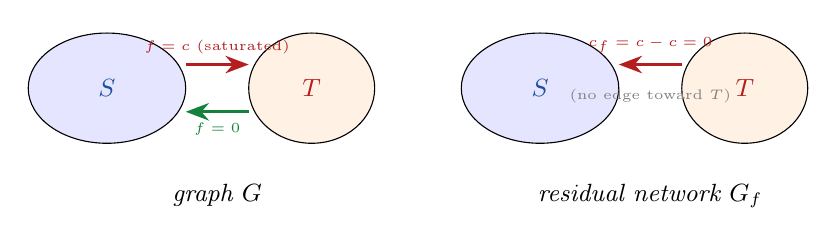
\begin{tikzpicture}[font=\small, >=Stealth,
    node/.style={circle, draw, fill=blue!8, minimum size=0.55cm, inner sep=1pt}]
  % Left: original graph with saturated/zero edges
  \begin{scope}[xshift=0cm]
    \node[draw, ellipse, fill=blue!10, minimum width=2cm, minimum height=1.4cm]
          at (0.4, 0) {};
    \node[font=\bfseries\small, keyblue] at (0.4, 0) {$S$};
    \node[draw, ellipse, fill=orange!10, minimum width=1.6cm, minimum height=1.4cm]
          at (3.0, 0) {};
    \node[font=\bfseries\small, keyred] at (3.0, 0) {$T$};
    \draw[->, keyred, very thick] (1.4, 0.3) -- node[above,font=\tiny,keyred]{$f=c$ (saturated)} (2.2, 0.3);
    \draw[->, keygreen, very thick] (2.2, -0.3) -- node[below,font=\tiny,keygreen]{$f=0$} (1.4, -0.3);
    \node[below=14pt] at (1.8, -0.6) {\textit{graph $G$}};
  \end{scope}
  % Right: residual network
  \begin{scope}[xshift=5.5cm]
    \node[draw, ellipse, fill=blue!10, minimum width=2cm, minimum height=1.4cm]
          at (0.4, 0) {};
    \node[font=\bfseries\small, keyblue] at (0.4, 0) {$S$};
    \node[draw, ellipse, fill=orange!10, minimum width=1.6cm, minimum height=1.4cm]
          at (3.0, 0) {};
    \node[font=\bfseries\small, keyred] at (3.0, 0) {$T$};
    \draw[->, keyred, very thick] (2.2, 0.3) -- node[above,font=\tiny,keyred]{$c_f = c-c = 0$} (1.4, 0.3);
    \node[below=14pt] at (1.8, -0.6) {\textit{residual network $G_f$}};
    \node[gray, font=\tiny] at (1.8, -0.1) {(no edge toward $T$)};
  \end{scope}
\end{tikzpicture}
\end{center}

Therefore:
\[
  |f| = f(S,T) = \sum_{\substack{u\in S\\v\in T}} f(u,v) - \sum_{\substack{u\in S\\v\in T}} f(v,u)
       = \sum_{\substack{u\in S\\v\in T}} c(u,v) - 0 = c(S,T).
\]

\textbf{$(3) \Rightarrow (1)$:} Since $|f| \le c(S,T)$ for any cut,
if $|f| = c(S,T)$ for a minimum cut, the flow cannot be improved. Thus $f$ is maximum.
\end{proof}

% ─────────────────────────────────────────────────────────────────────────────
\subsection{Illustration on the Example}

In the 7-node network (optimal flow $|f| = 29$), the minimum cut identified by
$S = \{s\} \cup \{\text{nodes reachable from }s\text{ in }G_f\}$ satisfies
$c(S,T) = 29$: the edges of the cut are exactly saturated, and no augmenting
path exists in $G_f$.

% ─────────────────────────────────────────────────────────────────────────────
\subsection{Lecture Summary}

\begin{tcolorbox}[colback=lightblue, colframe=keyblue, fonttitle=\bfseries,
                  title={Key Points – Flows and Cuts}]
\begin{itemize}[noitemsep]
  \item \textbf{Cut $(S,T)$}: partition $V = S \cup T$ with $s \in S$, $t \in T$.
  \item \textbf{Net Flow} $f(S,T) = \sum_{S \to T} f - \sum_{T \to S} f$.
  \item \textbf{Capacity} $c(S,T) = \sum_{u\in S, v\in T} c(u,v)$.
  \item \textbf{Fundamental Identity:} $|f| = f(S,T)$ for any cut,
        hence $|f| \le c(S,T)$.
  \item \textbf{Max-Flow Min-Cut Theorem:}
    \[
      \max |f| = \min c(S,T).
    \]
    Three equivalent conditions: max flow $\Leftrightarrow$ no augmenting
    path in $G_f$ $\Leftrightarrow$ flow equals min-cut capacity.
  \item \textbf{Ford-Fulkerson returns an optimal flow} because it stops
        precisely when condition (2) is verified.
\end{itemize}
\end{tcolorbox}

\section{Lecture 16 : Ford-Fulkerson complexity and Applications}
% ══════════════════════════════════════════════════════════════════════════════
% Lecture 16: Ford-Fulkerson Complexity and Applications
% ══════════════════════════════════════════════════════════════════════════════

% ══════════════════════════════════════════════════════════════════════════════
\section*{Complexity of the Ford-Fulkerson Method}
\addcontentsline{toc}{subsection}{Ford-Fulkerson Complexity}
% ══════════════════════════════════════════════════════════════════════════════

% ─────────────────────────────────────────────────────────────────────────────
\subsection{Upper Bound (Integer Capacities)}

\begin{complexity}{Ford-Fulkerson — Naive Bound}{ffnaive}
Assuming integer capacities:
\begin{itemize}[noitemsep]
  \item Finding an augmenting path in $G_f$ takes $O(E)$ (using BFS or DFS).
  \item In each iteration, the flow value increases by at least 1.
  \item \textbf{Total Complexity: $O(E \cdot |f_{\max}|)$} where $|f_{\max}|$ is the 
        maximum flow value.
\end{itemize}
\end{complexity}

This bound is correct but can be very poor if the capacities are large.

% ─────────────────────────────────────────────────────────────────────────────
\subsection{Problematic Case}

Consider the diamond graph with a central edge of capacity 1 and 
capacities $M = 2^{100}$ on the other edges:

\begin{center}
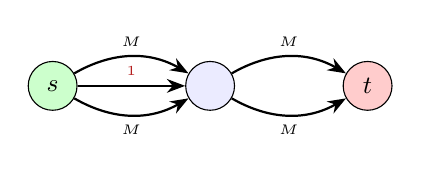
\begin{tikzpicture}[font=\small, >=Stealth,
    node/.style={circle, draw, fill=blue!8, minimum size=0.62cm, inner sep=1pt}]
  \node[node, fill=green!20] (s)  at (0, 1)   {$s$};
  \node[node]                (m)  at (2, 1)   {};
  \node[node, fill=red!20]   (t)  at (4, 1)   {$t$};
  \draw[->, thick] (s) to[bend left=30]  node[above,font=\tiny]{$M$}   (m);
  \draw[->, thick] (s) to[bend right=30] node[below,font=\tiny]{$M$}   (m);
  \draw[->, thick] (m) to[bend left=30]  node[above,font=\tiny]{$M$}   (t);
  \draw[->, thick] (m) to[bend right=30] node[below,font=\tiny]{$M$}   (t);
  \draw[->, thick] (s) -- node[above,font=\tiny,keyred]{$1$}            (m);
\end{tikzpicture}
\end{center}

If Ford-Fulkerson alternately chooses the top path and the bottom path 
by passing through the central edge (capacity 1), the flow increases by 1 
each time. It would take $2M = 2^{101}$ iterations to reach the optimum $|f_{\max}| = 2M$.

\begin{remark}{Irrational Capacities}{irrational}
If capacities are irrational, the Ford-Fulkerson method may 
\textbf{never terminate}: the sequence of flows may converge to a 
sub-optimal value.
\end{remark}

% ─────────────────────────────────────────────────────────────────────────────
\subsection{Variants with Good Complexity}

There are two augmenting path choices that guarantee efficient 
termination for integer capacities:

\begin{center}
\renewcommand{\arraystretch}{1.5}
\begin{tabular}{lcc}
\toprule
\textbf{Augmenting Path Choice} & \textbf{Number of Iterations} & \textbf{Implementation} \\
\midrule
\textbf{Shortest Path} (BFS) & $\le \dfrac{1}{2} \cdot |E| \cdot |V|$ & BFS \\[6pt]
\textbf{Fattest Path} & $\le |E| \cdot \log(|E| \cdot U)$ & Modified Dijkstra \\
\bottomrule
\end{tabular}
\end{center}

where $U$ is the maximum flow value.

\textbf{Shortest Path (Edmonds-Karp algorithm):} we choose an augmenting 
path with the \emph{fewest edges} possible (BFS) at each iteration. 
The total number of iterations is bounded by $O(|V| \cdot |E|)$, which 
gives a global complexity of $O(|V| \cdot |E|^2)$.

\textbf{Fattest Path:} we choose the augmenting path whose 
bottleneck capacity ($c_f(p) = \min_{(u,v)\in p} c_f(u,v)$) is 
\emph{maximal}. This choice eliminates the problematic case described above.

% ══════════════════════════════════════════════════════════════════════════════
\section*{Maximum Flow Applications}
\addcontentsline{toc}{subsection}{Maximum Flow Applications}
% ══════════════════════════════════════════════════════════════════════════════

% ─────────────────────────────────────────────────────────────────────────────
\subsection{Bipartite Matching}

\subsubsection{Problem}

$N$ students apply for $M$ job offers ($M \ge N$). Each student 
receives several offers. Can we find a matching that assigns each student 
to exactly one job for which they were accepted?

\begin{definition}{Bipartite Graph and Matching}{bipartite}
A \textbf{bipartite graph} $G = (L \cup R, E)$ has two disjoint 
vertex sets $L$ (students) and $R$ (jobs); all edges go from 
$L$ to $R$. A \textbf{matching} is a subset of edges such that each 
vertex is incident to at most one edge of the matching.
\end{definition}

\subsubsection{Reduction to Maximum Flow}

\begin{center}
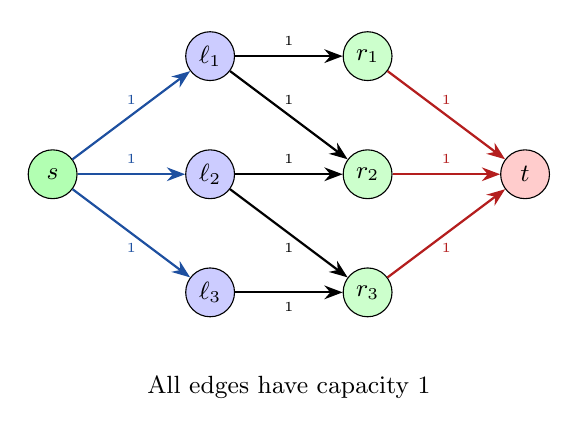
\begin{tikzpicture}[font=\small, >=Stealth,
    node/.style={circle, draw, fill=blue!8, minimum size=0.62cm, inner sep=1pt},
    student/.style={circle, draw, fill=blue!20, minimum size=0.62cm, inner sep=1pt},
    job/.style={circle, draw, fill=green!20, minimum size=0.62cm, inner sep=1pt}]
  \node[node, fill=green!30] (s) at (0, 2)   {$s$};
  \node[student] (l1) at (2, 3.5) {$\ell_1$};
  \node[student] (l2) at (2, 2)   {$\ell_2$};
  \node[student] (l3) at (2, 0.5) {$\ell_3$};
  \node[job]     (r1) at (4, 3.5) {$r_1$};
  \node[job]     (r2) at (4, 2)   {$r_2$};
  \node[job]     (r3) at (4, 0.5) {$r_3$};
  \node[node, fill=red!20]   (t) at (6, 2)   {$t$};

  % s -> students (capacity 1)
  \draw[->, thick, keyblue] (s)  -- node[above,font=\tiny]{1} (l1);
  \draw[->, thick, keyblue] (s)  -- node[above,font=\tiny]{1} (l2);
  \draw[->, thick, keyblue] (s)  -- node[below,font=\tiny]{1} (l3);

  % students -> jobs (capacity 1, preferences)
  \draw[->, thick] (l1) -- node[above,font=\tiny]{1} (r1);
  \draw[->, thick] (l1) -- node[above,font=\tiny]{1} (r2);
  \draw[->, thick] (l2) -- node[above,font=\tiny]{1} (r2);
  \draw[->, thick] (l2) -- node[below,font=\tiny]{1} (r3);
  \draw[->, thick] (l3) -- node[below,font=\tiny]{1} (r3);

  % jobs -> t (capacity 1)
  \draw[->, thick, keyred] (r1) -- node[above,font=\tiny]{1} (t);
  \draw[->, thick, keyred] (r2) -- node[above,font=\tiny]{1} (t);
  \draw[->, thick, keyred] (r3) -- node[below,font=\tiny]{1} (t);

  \node[below=4pt, font=\small] at (3, -0.3)
        {All edges have capacity 1};
\end{tikzpicture}
\end{center}

The construction is:
\begin{itemize}[noitemsep]
  \item Add source $s$ connected to each student (capacity 1).
  \item Add sink $t$ connected from each job (capacity 1).
  \item Direct student$\to$job edges (capacity 1).
  \item Run Ford-Fulkerson.
\end{itemize}

\begin{theorem}{Max Flow = Max Matching}{bipmatch}
The value of the maximum flow in this network is equal to the size of 
the maximum matching in the bipartite graph.
\end{theorem}

\begin{proof}
\textbf{Matching $\Rightarrow$ Flow.} Given a matching of size $k$, 
we construct a flow of value $k$ by setting 1 on the matching edges and 
on the corresponding $s$-student and job-$t$ edges.

\textbf{Flow $\Rightarrow$ Matching.} Since capacities are integers, 
Ford-Fulkerson produces an integer flow (0 or 1 on each edge). 
Flow conservation implies: each student receives at most 1 unit of flow 
from $s$, and each job sends at most 1 unit to $t$. The student$\to$job 
edges with flow 1 thus form a matching of size $|f|$.
\end{proof}

% ─────────────────────────────────────────────────────────────────────────────
\subsection{Edge-Disjoint Paths}

\subsubsection{Problem}

In winter, some roads may be closed. How many distinct routes 
(sharing no edges) exist between Lausanne ($s$) and Geneva airport ($t$)? 
What is the minimum number of roads that must be closed to block 
all traffic from $s$ to $t$?

\begin{definition}{Edge-Disjoint Paths}{edgedisj}
Two paths are \textbf{edge-disjoint} if they share no edge. 
The \textbf{maximum number of edge-disjoint paths} from $s$ to $t$ is the 
largest set of pairwise edge-disjoint $s \leadsto t$ paths.
\end{definition}

\subsubsection{Reduction to Maximum Flow}

We build a flow network from the road graph:
\begin{itemize}[noitemsep]
  \item Assign a capacity of 1 to each road (in each direction).
  \item Remove anti-parallel edges via the dummy vertex gadget $v'$ 
        (seen in Lecture 14).
  \item Run Ford-Fulkerson.
\end{itemize}

\begin{tcolorbox}[colback=lightgreen, colframe=keygreen, fonttitle=\bfseries,
                  title={Flow/Cut Duality for Edge-Disjoint Paths}]
\[
  \text{max-flow} = \text{maximum number of edge-disjoint paths}
\]
\[
  \text{min-cut} = \text{minimum number of roads to close to isolate }s\text{ from }t
\]
\end{tcolorbox}

The minimum cut identifies exactly the minimal set of roads whose 
closure blocks every path from Lausanne to Geneva.

% ─────────────────────────────────────────────────────────────────────────────
\subsection{Lecture Summary}

\begin{tcolorbox}[colback=lightblue, colframe=keyblue, fonttitle=\bfseries,
                  title={Key Points}]
\begin{itemize}[noitemsep]
  \item \textbf{Naive Complexity:} $O(E \cdot |f_{\max}|)$ — can be exponential 
        if capacities are large or irrational.
  \item \textbf{Edmonds-Karp (BFS):} $\le \frac{1}{2} |E| \cdot |V|$ iterations, 
        thus $O(|V| \cdot |E|^2)$ total.
  \item \textbf{Fattest Path:} $\le |E| \cdot \log(|E| \cdot U)$ iterations.
  \item \textbf{Bipartite Matching:} reduction to capacity-1 flow network; 
        max flow $=$ max matching (integrality guaranteed by Ford-Fulkerson).
  \item \textbf{Edge-Disjoint Paths:} capacity 1 on each edge; 
        max flow $=$ number of edge-disjoint paths; 
        min cut $=$ min number of edges to remove.
\end{itemize}
\end{tcolorbox}

\section{Lecture 17: Disjoint set and minimum spanning trees}
 % ══════════════════════════════════════════════════════════════════════════════
% Lecture 17: Union-Find and Minimum Spanning Trees
% ══════════════════════════════════════════════════════════════════════════════

% ══════════════════════════════════════════════════════════════════════════════
\section*{Disjoint-Set Data Structures (Union-Find)}
\addcontentsline{toc}{subsection}{Union-Find Data Structure}
% ══════════════════════════════════════════════════════════════════════════════

% ─────────────────────────────────────────────────────────────────────────────
\subsection{Introduction}

\begin{definition}{Disjoint-Set Data Structure}{disjointset}
A \textbf{disjoint-set data structure} (also known as \textbf{union-find}) maintains a collection 
$\mathcal{S} = \{S_1, S_2, \ldots, S_k\}$ of disjoint dynamic sets. Each set is identified by 
a \textbf{representative}, which is some member of the set. The representative doesn't matter 
as long as querying the representative twice without modifying the set returns the same answer.
\end{definition}

The union-find data structure supports three fundamental operations:

\begin{itemize}[noitemsep]
  \item \textbf{Make-Set}$(x)$: Create a new set $S_i = \{x\}$ and add $S_i$ to $\mathcal{S}$.
  \item \textbf{Union}$(x, y)$: If $x \in S_x$ and $y \in S_y$, replace $S_x$ and $S_y$ with 
        $S_x \cup S_y$ in $\mathcal{S}$. The representative of the new set is any member in 
        $S_x \cup S_y$ (often the representative of one of $S_x$ or $S_y$). This operation 
        destroys $S_x$ and $S_y$ since sets must remain disjoint.
  \item \textbf{Find}$(x)$: Return the representative of the set containing $x$.
\end{itemize}

% ─────────────────────────────────────────────────────────────────────────────
\subsection{Application: Connected Components}

A classic application of union-find is computing connected components in an undirected graph 
$G = (V, E)$. Two vertices $u$ and $v$ are in the same connected component if and only if 
there is a path between them. Connected components partition vertices into equivalence classes.

The algorithm proceeds as follows:
\begin{itemize}[noitemsep]
  \item Initialize: For each vertex $v \in V$, call Make-Set$(v)$.
  \item For each edge $(u, v) \in E$: if Find$(u) \neq$ Find$(v)$, call Union$(u, v)$.
\end{itemize}

This requires $|V|$ Make-Set operations, at most $2|E|$ Find operations, and at most $|V|-1$ 
Union operations, for a total of at most $|V| + 3|E|$ operations.

% ─────────────────────────────────────────────────────────────────────────────
\subsection{Linked List Representation}

One implementation represents each set as a singly linked list:
\begin{itemize}[noitemsep]
  \item Each set object maintains a pointer to the head (the representative) and the tail.
  \item Each list element contains the set member, a pointer to the next element, and a 
        pointer back to the set object.
\end{itemize}

\textbf{Operations:}
\begin{itemize}[noitemsep]
  \item Make-Set$(x)$: Create a singleton list in time $\Theta(1)$.
  \item Find$(x)$: Follow the pointer to the set object, then to the representative in $\Theta(1)$.
  \item Union$(x, y)$: Append $y$'s list onto the end of $x$'s list using $x$'s tail pointer. 
        Update the set pointer for every element in $y$'s list. This can take $\Theta(n)$ time 
        in the worst case.
\end{itemize}

\textbf{Weighted-Union Heuristic:} Always append the smaller list to the larger list (break ties arbitrarily).

\begin{theorem}{Linked List with Weighted-Union}{linkedlistuf}
With the weighted-union heuristic, a sequence of $m$ operations (Make-Set, Union, Find) on 
$n$ elements takes $O(m + n \log n)$ time.
\end{theorem}

\begin{proof}
Make-Set and Find still take constant time. The key observation is: how many times can each 
element's representative pointer be updated? Each time an element's pointer is updated, it must 
be in the smaller set being appended to a larger set. Thus the size of the set containing that 
element at least doubles. Since the maximum set size is $n$, each element's pointer can be 
updated at most $\log n$ times. With $n$ elements and at most $n$ unions, the total cost of 
all pointer updates is $O(n \log n)$.
\end{proof}

For the connected components problem with $|V|$ elements and $\le |V| + 3|E|$ operations, 
the total running time is $O(|V| \log |V| + |E|)$.

% ─────────────────────────────────────────────────────────────────────────────
\subsection{Disjoint-Set Forest}

A more efficient implementation represents each set as a rooted tree:
\begin{itemize}[noitemsep]
  \item Each node $x$ has a parent pointer $x.p$.
  \item The root of each tree is the representative of the set.
  \item Each node also maintains a rank $x.\text{rank}$ (an upper bound on the height).
\end{itemize}

\textbf{Operations:}

\begin{algorithm}[H]
\caption{Make-Set and Find-Set}
\begin{algorithmic}[1]
\Procedure{Make-Set}{$x$}
  \State $x.p \gets x$
  \State $x.\text{rank} \gets 0$
\EndProcedure
\end{algorithmic}
\begin{algorithmic}[1]
\Procedure{Find-Set}{$x$}
  \If{$x \neq x.p$}
    \State $x.p \gets$ \Call{Find-Set}{$x.p$} \AlgComment{Path compression}
  \EndIf
  \State \Return $x.p$
\EndProcedure
\end{algorithmic}
\end{algorithm}

\begin{algorithm}[H]
\caption{Union by Rank}
\begin{algorithmic}[1]
\Procedure{Union}{$x, y$}
\State \Call{Link}{\text{Find-Set}(x), \text{Find-Set}(y)}
\EndProcedure

\Statex % Adds a small gap between procedures

\Procedure{Link}{$x, y$}
    \If{$x.\text{rank} > y.\text{rank}$}
        \State $y.p \gets x$
    \Else
        \State $x.p \gets y$
        \If{$x.\text{rank} = y.\text{rank}$}
            \State $y.\text{rank} \gets y.\text{rank} + 1$
        \EndIf
    \EndIf
\EndProcedure
\end{algorithmic}
\end{algorithm}

\textbf{Union by rank:} Always attach the tree with smaller rank under the root of the tree 
with larger rank.

\textbf{Path compression:} During Find-Set$(x)$, make each node on the path from $x$ to the 
root point directly to the root.

\begin{complexity}{Forest with Union-by-Rank and Path Compression}{forestuf}
If we use both union by rank and path compression, a sequence of $m$ operations (Make-Set, 
Union, Find) on $n$ elements takes $O(m \cdot \alpha(n))$ time, where $\alpha(n)$ is the 
\textbf{inverse Ackermann function}.
\end{complexity}

\begin{remark}{Inverse Ackermann Function}{invack}
The function $\alpha(n)$ is an extremely slowly growing function. For all practical purposes, 
$\alpha(n) \le 4$:
\begin{center}
\begin{tabular}{cc}
\toprule
$n$ & $\alpha(n)$ \\
\midrule
$0$ to $2$ & $0$ \\
$3$ & $1$ \\
$4$ to $7$ & $2$ \\
$8$ to $2047$ & $3$ \\
$2048$ to $A(4,2)$ & $4$ \\
\bottomrule
\end{tabular}
\end{center}
where $A(4,2)$ is a number with more than $10^{19000}$ digits. Thus, for the connected 
components problem, the running time is $O((|V| + |E|) \alpha(|V|)) \approx O(|V| + |E|)$, 
which is essentially linear.
\end{remark}

% ══════════════════════════════════════════════════════════════════════════════
\section*{Minimum Spanning Trees}
\addcontentsline{toc}{subsection}{Minimum Spanning Trees}
% ══════════════════════════════════════════════════════════════════════════════

% ─────────────────────────────────────────────────────────────────────────────
\subsection{Problem Definition}

\begin{definition}{Minimum Spanning Tree (MST)}{mst}
\textbf{Input:} An undirected, connected graph $G = (V, E)$ with a weight function 
$w: E \to \mathbb{R}$ that assigns a weight $w(u,v)$ to each edge $(u,v) \in E$.

\textbf{Output:} A spanning tree $T \subseteq E$ of minimum total weight 
$w(T) = \sum_{(u,v) \in T} w(u,v)$.

A \textbf{spanning tree} is an acyclic subset of edges that connects all vertices. 
It has exactly $|V| - 1$ edges.
\end{definition}

% ─────────────────────────────────────────────────────────────────────────────
\subsection{Applications}

\textbf{Communication Networks:} A multinational company wants to lease communication lines 
between its various locations. Each pair of locations has a cost for leasing a direct line. 
The company wants to connect all locations with minimum total cost. The solution is the 
minimum spanning tree of the graph where vertices are locations and edge weights are 
leasing costs.

% ─────────────────────────────────────────────────────────────────────────────
\subsection{Generic Greedy Approach}

Both Kruskal's and Prim's algorithms are based on a generic greedy strategy. The key 
theoretical tool is the \textbf{cut property}.

\begin{definition}{Cut}{cut}
A \textbf{cut} $(S, V \setminus S)$ is a partition of the vertices into two disjoint sets 
$S$ and $V \setminus S$. An edge $(u,v)$ \textbf{crosses} the cut if one endpoint is in $S$ 
and the other is in $V \setminus S$.
\end{definition}

\begin{theorem}{Cut Property (Safe Edge Theorem)}{cutprop}
Consider a cut $(S, V \setminus S)$ and let:
\begin{itemize}[noitemsep]
  \item $T$ be a tree on $S$ which is part of some MST
  \item $e$ be a crossing edge of minimum weight
\end{itemize}
Then there exists an MST of $G$ containing both $e$ and $T$.
\end{theorem}

\begin{proof}
If $e$ is already in the MST, we are done. Otherwise, add $e$ to the MST. This creates a 
cycle with at least one other crossing edge $f$ (since the MST was already spanning). 
We have $w(f) \ge w(e)$ since $e$ is a minimum weight crossing edge. Replace $f$ by $e$ 
in the MST. The total weight doesn't increase: $w(\text{new MST}) = w(\text{old MST}) - w(f) + w(e) \le w(\text{old MST})$. 
Thus the new tree is also an MST, and it contains both $T$ and $e$.
\end{proof}

% ─────────────────────────────────────────────────────────────────────────────
\subsection{Prim's Algorithm}

\textbf{Idea:} Start with an arbitrary vertex $v$ and set $T = \{v\}$. Greedily grow the 
tree $T$: at each step, add to $T$ a minimum-weight crossing edge with respect to the cut 
$(T, V \setminus T)$.

\textbf{Correctness:} At each iteration, by the cut property, the minimum crossing edge is 
safe to add. The algorithm terminates when $T$ is a spanning tree.

\textbf{Implementation Challenge:} How do we find the minimum crossing edge at every iteration?

\begin{itemize}[noitemsep]
  \item \textbf{Naive approach:} Check all outgoing edges. This requires $O(|E|)$ comparisons 
        at each iteration, giving $O(|E| \cdot |V|)$ total time.
  \item \textbf{Efficient approach:} For every vertex $w \notin T$, maintain $\text{dist}(w)$, 
        the weight of the lightest edge from $w$ to any vertex in $T$. When a new vertex $u$ 
        is added to $T$, check whether neighbors of $u$ decrease their distance to $T$. Use a 
        min-priority queue to extract the vertex with minimum distance.
\end{itemize}

\begin{complexity}{Prim's Algorithm}{prim}
With a binary min-heap, Prim's algorithm runs in $O(|E| \log |V|)$ time:
\begin{itemize}[noitemsep]
  \item $|V|$ Extract-Min operations: $O(|V| \log |V|)$
  \item At most $|E|$ Decrease-Key operations: $O(|E| \log |V|)$
\end{itemize}
With a Fibonacci heap, the time improves to $O(|E| + |V| \log |V|)$.
\end{complexity}

% ─────────────────────────────────────────────────────────────────────────────
\subsection{Kruskal's Algorithm}

\textbf{Idea:} Start with an empty forest $T$. Sort all edges by weight in non-decreasing 
order. Greedily add the cheapest edge that does not create a cycle.

\begin{algorithm}[H]
\caption{Kruskal's MST Algorithm}
\begin{algorithmic}[1]
\Procedure{MST-Kruskal}{$G, w$}
  \State $A \gets \emptyset$
  \For{each vertex $v \in V$}
    \State \Call{Make-Set}{$v$} \AlgComment{Initialize disjoint sets}
  \EndFor
  \State Sort edges of $E$ by weight in non-decreasing order
  \For{each edge $(u, v) \in E$ in sorted order}
    \If{\Call{Find-Set}{$u$} $\neq$ \Call{Find-Set}{$v$}}
      \State $A \gets A \cup \{(u, v)\}$ \AlgComment{Add edge to MST}
      \State \Call{Union}{$u, v$}
    \EndIf
  \EndFor
  \State \Return $A$
\EndProcedure
\end{algorithmic}
\end{algorithm}

\textbf{Correctness:} The algorithm maintains the invariant that $T$ is always a sub-forest 
of some MST. When we add edge $(u, v)$, the endpoints are in different connected components. 
Consider the cut $(S, V \setminus S)$ where $S$ is the component containing $u$. Since $(u, v)$ 
is the cheapest remaining edge and it crosses this cut, by the cut property, it is safe to add.

\textbf{Implementation Challenge:} We need to check whether adding edge $(u, v)$ creates a 
cycle. This is equivalent to checking whether $u$ and $v$ are already in the same connected 
component. This is exactly what the union-find data structure provides.

\begin{complexity}{Kruskal's Algorithm}{kruskal}
Analysis of Kruskal's algorithm:
\begin{itemize}[noitemsep]
  \item Initialize $A$: $O(1)$
  \item First for loop: $|V|$ Make-Set operations
  \item Sort edges: $O(|E| \log |E|)$
  \item Second for loop: $O(|E|)$ Find-Set and Union operations
  \item Total union-find operations: $O((|V| + |E|) \alpha(|V|))$
\end{itemize}
Total time: $O((|V| + |E|) \alpha(|V|)) + O(|E| \log |E|) = O(|E| \log |E|) = O(|E| \log |V|)$ 
(since $|E| \le |V|^2$, we have $\log |E| = O(\log |V|)$).

If edges are already sorted, the time becomes $O(|E| \alpha(|V|))$, which is almost linear.
\end{complexity}

% ─────────────────────────────────────────────────────────────────────────────
\subsection{Lecture Summary}

\begin{tcolorbox}[colback=lightblue, colframe=keyblue, fonttitle=\bfseries,
                  title={Key Points}]
\begin{itemize}[noitemsep]
  \item \textbf{Union-Find Data Structure:} maintains disjoint sets with operations Make-Set, 
        Union, and Find. Essential for tracking connected components.
  \item \textbf{Linked list implementation:} $O(m + n \log n)$ time for $m$ operations on 
        $n$ elements with weighted-union heuristic.
  \item \textbf{Forest implementation:} $O(m \cdot \alpha(n))$ time with union-by-rank and 
        path compression, where $\alpha(n)$ is the inverse Ackermann function (practically constant).
  \item \textbf{MST Problem:} Find a spanning tree of minimum total weight in a weighted 
        undirected graph.
  \item \textbf{Cut Property:} The minimum weight crossing edge is safe to add to any partial MST.
  \item \textbf{Prim's Algorithm:} Grow the tree from a single vertex by repeatedly adding 
        the minimum crossing edge. Time: $O(|E| \log |V|)$ with binary heap.
  \item \textbf{Kruskal's Algorithm:} Sort edges and add the cheapest edge that doesn't create 
        a cycle using union-find. Time: $O(|E| \log |V|)$ (sorting dominates).
  \item Both algorithms are greedy and produce correct MSTs by the cut property.
\end{itemize}
\end{tcolorbox}
\end{document}